\documentclass[10pt]{article}
\usepackage[utf8]{inputenc}
\usepackage{empheq}
\usepackage[inline, shortlabels]{enumitem}
\usepackage{gensymb}
\usepackage{multicol}
\setlength{\parskip}{0.5cm plus4mm minus3mm}
\setlength{\parindent}{0pt}
\usepackage{amsmath}
\usepackage{upgreek}
\usepackage{tikz}
\usepackage{wrapfig}
\usepackage[nobreak=true]{mdframed}
\usepackage[margin=0.6in]{geometry}
 \geometry{
 left=12mm,
 bottom=20mm
 }
\usepackage{amssymb}
\usepackage{cs170}
\usepackage{titlesec}
\usepackage{chngcntr}
\usepackage{graphicx}
\usepackage{changepage}
\usepackage{chngcntr}
\usepackage{scrextend}
\usepackage{minted}
\usemintedstyle{colorful}

\begin{document}
\date{}
\author{}
\title{\vspace{-5ex} \dunhd{CS170: Algorithms Notes} \vspace{-5ex}}
\maketitle


\begin{multicols}{2}
\section{Prologue}
\begin{addmargin}[0.8em]{0.5em}
    \subsection{Big O Notation}
    \begin{enumerate}[label=(\alph*)]
        \item While it is possible to express running time in terms of basic computer operations, accounting for architecture-specific minutiae yields a result that does not generalize from one computer to the next. A better idea is to analyze running time by counting the number of basic computer operations \textit{as a function of the input size}.
        \item Let $f(n), g(n) : \mathbb{Z^+} \mapsto \mathbb{R}$. We say $f= O(g)$ if there exists $c>0$ such that $f(n) \leq c \cdot g(n)$.
        \item In other words, Big-O notation means $f(n)$ is less than or equal to $g(n)$, disregarding multiplicative constants and non-dominating terms.
        \item Big-O notation uses the following guidelines:
        \begin{enumerate}[label=(\roman*)]
            \item Omit constants (e.g. $14n^2 \rightarrow n^2$).
            \item $n^a$ dominates $n^b$ if $a > b$.
            \item Any exponential dominates any polynomial (e.g. $2^n$ dominates $n^5$).
            \item Any polynomial dominates any logarithm (e.g. $n$ dominates $\log(n)^3)$.
        \end{enumerate}
        \item Just as $O(\cdot)$ is an analog of $\leq$, $\Omega(\cdot)$ is an analog of $\geq$ and $\Theta(\cdot)$ is an analog of $=$. If $f = O(g)$  and $f = \Omega(g)$, then $f = \Theta(g)$.
    \end{enumerate}
    
    \subsection{Useful Identities and Series}
    \begin{enumerate}[label=(\alph*)]
        \item Logarithm Properties:
        \begin{enumerate}[label=(\roman*)]
            \item $y = \log_b(x)$ iff $x = b^y$
            \item $\log_b(xy) = \log_b(x) + \log_b(y)$
            \item $\log_b(x) = \log_c(x) / \log_c(b)$
            \item $\log_b(x^n) = n\log_b(x)$
            \item $x^{\log_b(y)} = y^{\log_b(x)}$
            \item $b^{\log_b{x}} = x$
        \end{enumerate}
        \item Basic Series:
        \begin{enumerate}
            \item $\sum_{k=1}^{n} k = \frac{n(n+1)}{2}$
            \item $\sum_{k=1}^{n} 2k - 1 = n^2$
            \item $\sum_{k=1}^{n} k^2 = \frac{n(n+1)(2n+1)}{6}$
            \item $\sum_{k=1}^{n} a r^{k-1} = \frac{a(1-r^n)}{1-r}$
            \item $\sum_{k=1}^{\infty} a r^{k-1} = \frac{a}{1-r}$, if  $|r| < 1$
            \item In big-$\Theta$ terms, the sum of a geometric series is the first term if the series is strictly decreasing, the last term if it's strictly increasing, or the number of terms if it's unchanging.
        \end{enumerate}
        
    \end{enumerate} 
\end{addmargin}

\section{Divide-and-Conquer Algorithms}
\begin{addmargin}[0.8em]{0.5em}
    \subsection{Recurrence Relations}
    \begin{enumerate}[label=(\alph*)]
        \item Divide-and-conquer algorithms often follow a generic pattern: they tackle a problem of size $n$ by recursively solving $a$ subproblems of size $\frac{n}{b}$ and then combining these answers in $O(n^d)$ time, for some $a, b, d > 0$. A problem of this form has running time $T(n) = aT(\lceil \frac{n}{b} \rceil) + O(n^d)$.
        \item \textbf{Master Theorem:} If $T(n) = aT(\lceil \frac{n}{b} \rceil) + O(n^d)$ for some $a > 0, b > 1$, and $d \geq 0$, then
        \begin{align*}
            T(n) = 
            \left\{
            \begin{array}{lr}
            O(n^d)           & \text{if } d > \log_b(a) \\
            O(n^d\log{n})    & \text{if } d = \log_b(a) \\
            O(n^{\log_b{a}}) & \text{if } d < \log_b(a)
            \end{array}
            \right.
        \end{align*}
        \vspace{-5pt}
        \begin{align*}
        \hspace{-7pt}
            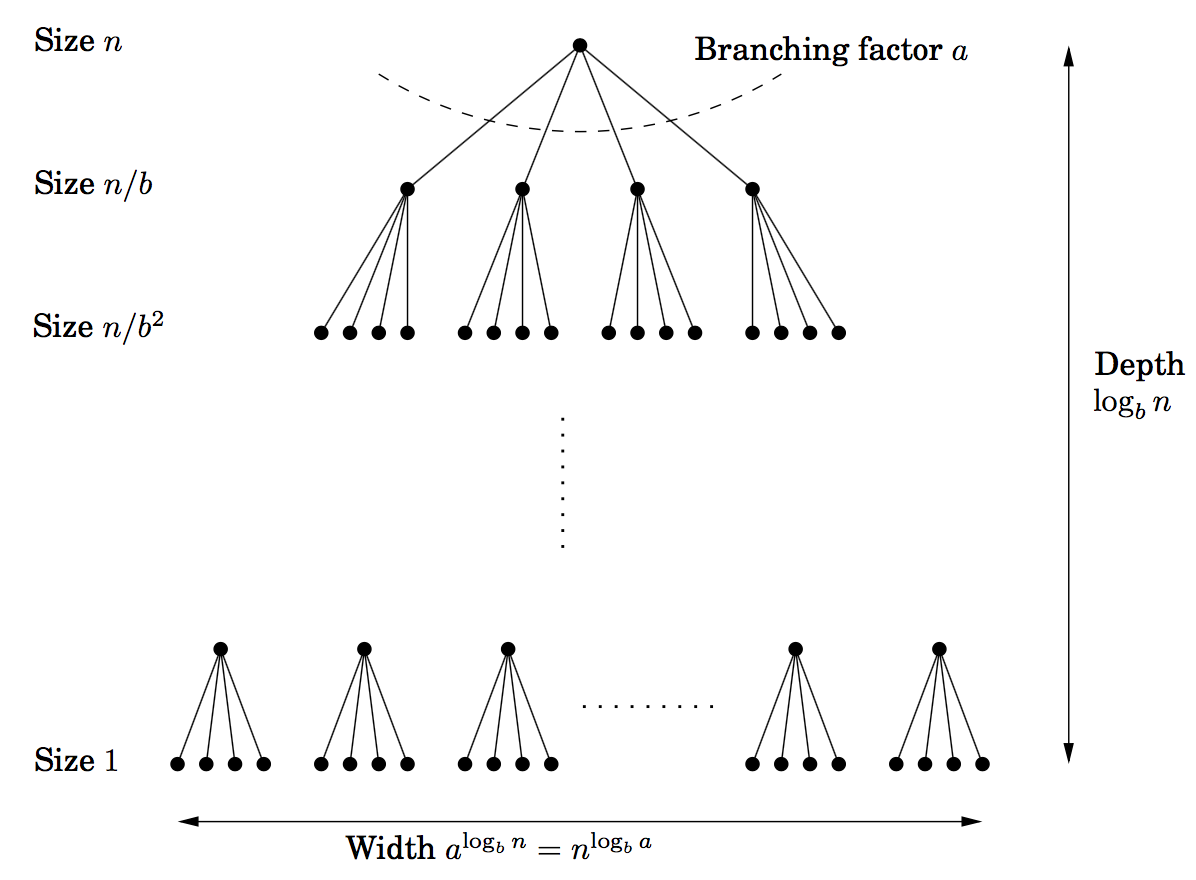
\includegraphics[width=6cm]{masterthm_tree.png}
        \end{align*}
        \vspace{-20pt}
        
        \item A more general version of the master theorem states if $T(n) = aT(\lceil \frac{n}{b} \rceil) + f(n)$ where $a \geq 1$, $b > 1$, and $f(n) = \Theta(n^c \log^k n)$ where $c = \log_b a$, then $$T(n) = \Theta(n^c \log^{k+1} n)$$
        
        \item For example, \textit{binary search} follows the recurrence with $a = 1, b = 2, d = 0$, which yields the familiar run time $O(\log(n))$. \textit{Mergesort}, which works by splitting a list into two halves, recursively sorting each half, then merging the two sorted sublists, has run time $O(n\log(n))$ since the merge operations are linear. An iterative version of mergesort is given below.
        
        \begin{minted}[linenos=false, escapeinside=||, mathescape=true]{octave}
function iterativeMergesort(|$a$|) 
Q = [ ] # empty queue 
for |$i = 1$| to |$n$|:
    Q.enqueue(|$a[i]$|) 
while Q.size() > 1:
    Q.enqueue(merge(Q.pop(), Q.pop()))
return Q.pop()
        \end{minted}
        
        \item A permutation tree argument shows that any comparison-based sorting algorithm must make $\Omega(n\log(n))$ comparisons. However, linear time sorting is possible on integers in a small range.
    \end{enumerate}
    
    \subsection{Arithmetic}
    \begin{enumerate}[label=(\alph*)]
        \item Addition and subtraction of $n$-bit numbers can be done in $O(n)$ time.
        \item Multiplication: Observe an $n$-bit number $x$ can be written $x=2^\frac{n}{2}x_L+x_R$, where $x_L$ and $x_R$ refer to the $n/2$-bit halves of $x$. To compute $xy$, the product of two $n$-bit integers, $xy = (2^\frac{n}{2}x_L+x_R)(2^\frac{n}{2}y_L+y_R) = 2^nx_Ly_L + 2^\frac{n}{2} (x_Ly_R + x_Ry_L) + x_Ry_R$. The additions and multiplications by powers of 2 (which are merely left-shifts) take linear time. The four $n/2$-bit multiplications can be done recursively. 
        \item By the master theorem, $T(n) = 4T(n/2)+O(n)$ and the runtime is $O(n^2)$. Gauss’s trick uses clever algebra to reduce the number of $n/2$-bit multiplciations to 3, which reduces the runtime to $O(n^{1.59})$.
        \item Matrix multiplication: By splitting an $n\times n$ matrix into four $\frac{n}{2} \times \frac{n}{2}$ submatrices, the product of two $n\times n$ matrices can be expressed as eight $\frac{n}{2} \times \frac{n}{2}$ matrix products with $O(n^2)$ additions, which has $O(n^3)$ runtime. Strassen's clever algebra trick reduced the number of matrix multiplications to 7, resulting in a runtime of $O(n^{2.81})$. In practice, Strassen's algorithm is very commonly used.
    \end{enumerate}       
    
    \subsection{Selection}
    \begin{enumerate}[label=(\alph*)]
        \item Consider the problem of finding the $k^{th}$ smallest element of a set of numbers $S$ (e.g. $k=\lfloor |S|/2 \rfloor$ is the median). We have the following quicksort-inspired algorithm:
        \begin{minted}[linenos=false, escapeinside=??, mathescape=true]{octave}
function selection(?$S, k$?)
v = random(?$S$?)
?$S_L \hspace{0.8pt}= \{ a_i \mid a_i \in S, a_i < v \}$?
?$S_v \hspace{2pt}= \{ a_i \mid a_i \in S, a_i = v \}$?
?$S_R = \{ a_i \mid a_i \in S, a_i > v \}$?
if ?$k \leq |S_L|$?
    return selection(?$S_L, k$?)
if ?$|S_L| < k \leq |S_L| + |S_v|$?
    return v
if ?$k > |S_L| + |S_v|$?
    return selection(?$S_R, k - |S_L| - |S_v|$?) 
        \end{minted}        
        
    \item The runtime of this algorithm depends on the random choice of $v$. Call $v$ ``good" if it lies within the 25th to 75th percentile of the set $S$. If a good pivot is chosen, the next set will shrink to \textit{at most} three-fourths of its original size. 
    \item We have the recurrence relation (Time taken on set size $n$) $\leq$ 
    (Time taken on set size $\frac{3n}{4}$) + 
    (Time to reduce set size to $\frac{3n}{4}$). Taking the expectation of both sides, we have $T(n) \leq T(\frac{3n}{4}) + 2n$ (the factor of 2 because the last term has a geometric dristribution). From the master theorem, this has runtime $O(n)$ on average.
    \end{enumerate}     
    
    \subsection{Discrete Fourier Transform}
    \begin{enumerate}[label=(\alph*)]
        \item The Discrete Fourier Transform (DFT) is a linear transformation that converts a finite sequence of equally-spaced samples of a function into a sequence of equally-spaced samples of a complex-valued function of its frequency. It is widely used in signal processing, image processing, data compression, and many other fields. 
        \item Aside: for any $z=a+bi \in \mathbb{C}$, Euler's formula gives $z=a+bi=re^{i\theta}$, where $r=\sqrt{a^2+b^2}$ and $\tan{\theta} = \frac{b}{a}$.
        \item If $\vec{x} \in \mathbb{C}^n$, the DFT is $M_n(\omega)\vec{x}$, where $M_n(\omega)$ is the $n\times n$ unitary matrix
        \begin{align*}
        \begin{bmatrix}
        1 & 1 & 1 & \hdots & 1 \\
        1 & \omega & \omega^2 & \hdots & \omega^{n-1} \\
        \vdots & \vdots & \vdots & \ddots & \vdots \\
        1 & \omega^{n-1} & \omega^{2(n-1)} & \hdots & \omega^{(n-1)(n-1)}
        \end{bmatrix}
        \end{align*}
        where $\omega$ is the \textit{primitive} $n$th root of unity, equal to $e^{2\pi i / n}$. Recall the $nth$ roots of unity are the solutions to $z^n=1$, of which there are $n$: $1, \omega, \omega^2, \hdots, \omega^{n-1}$.
        \item $M_n(\omega)$ can be thought of as a change-of-coordinates matrix into the Fourier basis, or frequency domain. The inverse is $\frac{1}{n}M_n(\omega^{-1})$.
        \item Let $A(x) = a_0 + a_1x + \hdots + a_{n-1}x^{n-1}$. If 
        \begin{align*}
        \vec{x} = 
        \begin{bmatrix} a_0 \\ a_1 \\ \vdots \\ a_{n-1} \end{bmatrix} \text{, observe that } 
        M_n(\omega) \vec{x} = 
        \begin{bmatrix} A(0) \\ A(\omega) \\ \vdots \\ A(\omega^{n-1}) \end{bmatrix}.
        \end{align*}
        Thus, in the context of polynomials, the DFT takes a vector in the coefficient representation of a polynomial and returns an evaluation representation of the polynomial at the $n$th roots of unity.
    \end{enumerate}
\subsection{Fast Fourier Transform}
    \begin{enumerate}[label=(\alph*)]
        \item Whereas straightforward matrix-vector multiplication takes $O(n^2)$ operations, the Fast Fourier Transform (FFT) is a way to perform the DFT faster, in $O(n\log{n})$ operations.
        \item The idea is to evaluate $A(x)$ at the $n$th roots of unity by splitting the polynomial into its even $A_e(x)$ and odd $A_o(x)$ terms, such that $A(x) = A_e(x^2) + xA_o(x^2)$. The $n$th roots of unity are postive-negative pairs, so that the calculation of $A(x_i)$ can be recycled toward $A(-x_i)$:
        \begin{align*}
        A(x_i) &= A_e(x_i^2) + x_iA_o(x_i^2) \\
        A(-x_i) &= A_e(x_i^2) - x_iA_o(x_i^2) 
        \end{align*}
        \item The reason the $n$th roots of unity are used is so that we can recursively evaluate the two smaller polynomials $A_e(x)$ and $A_o(x)$ at the $(n/2)$th roots of unity (since the squares of the $n$th roots of unity become the $(n/2)$th roots of unity, which are still positive-negative paired). It recurses until it reaches the base case of evaluating $n$ polynomials at the single point $\omega^0=1$, at which point it returns $A(1)$.
        \item Using this strategy, the recursive step in the matrix-vector formulation for computing the vector $M_n(\omega)\vec{x}$ is as follows:
        \begin{align*}
        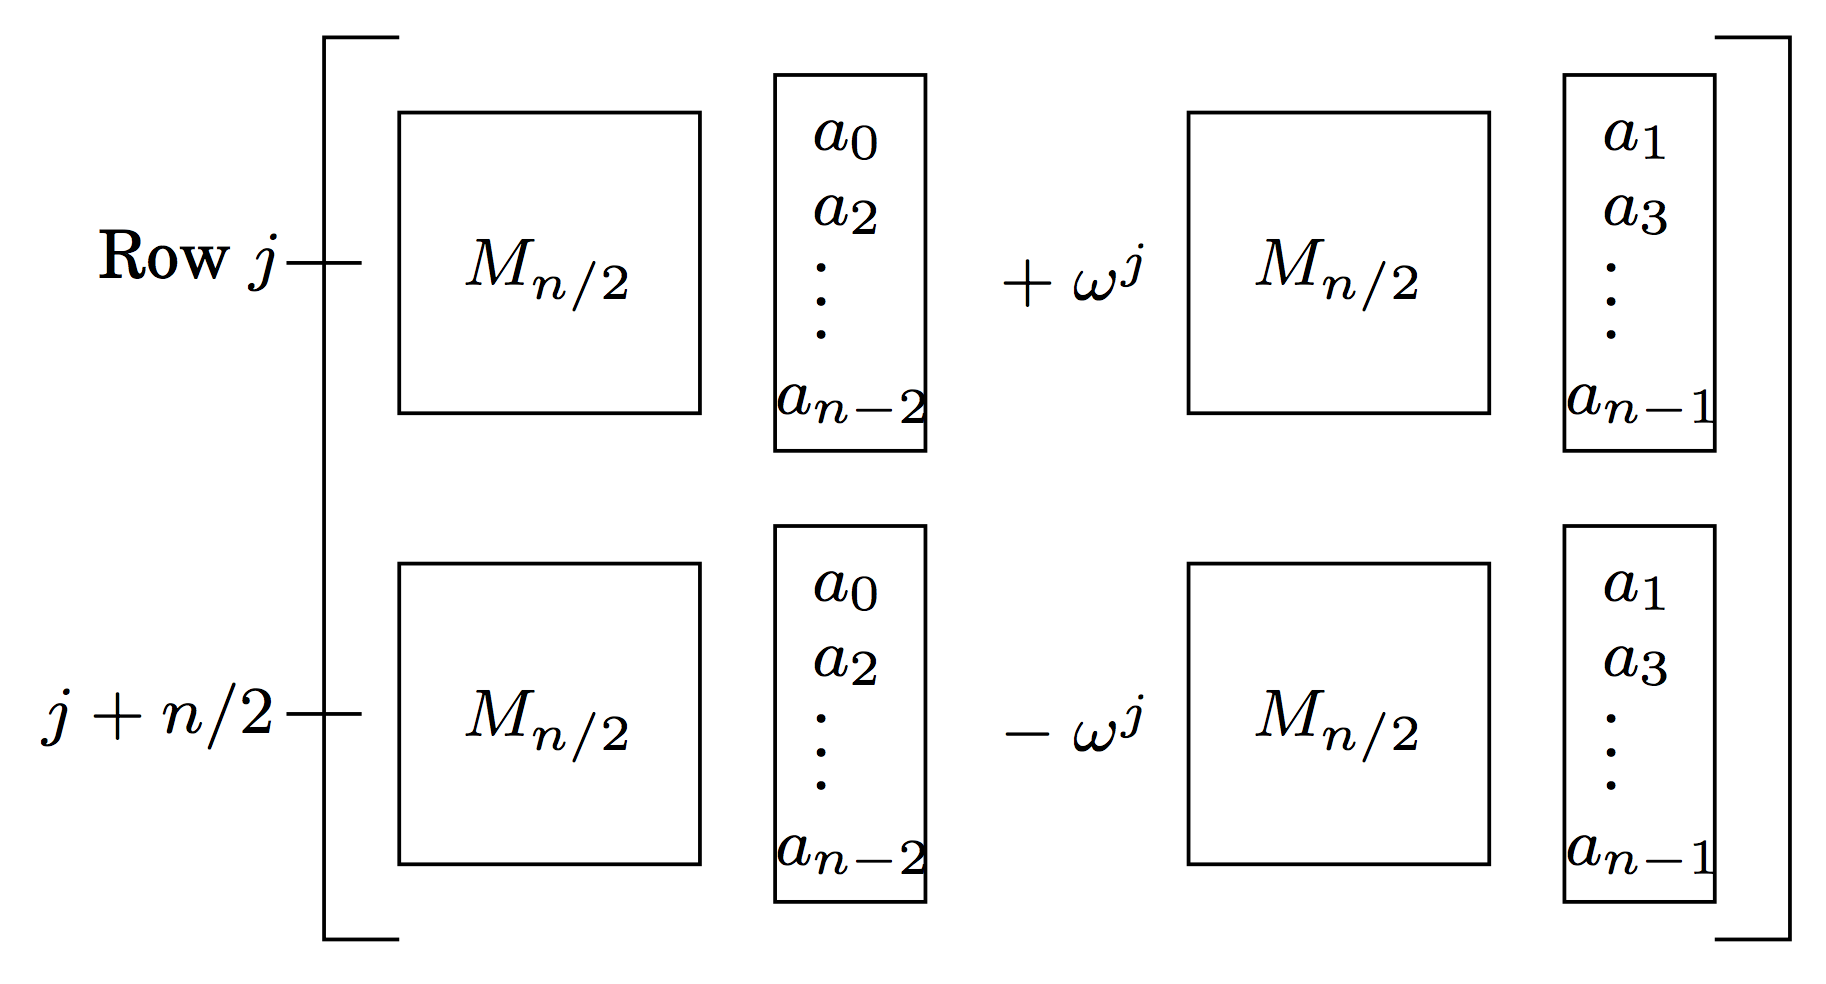
\includegraphics[width=6cm]{fft.png}
        \end{align*}
        In short, the product of $M_n(\omega)$ with vector $\vec{x}$, a size-$n$ problem, can be expressed in terms of two size-$n/2$ problems: the product of $M_{n/2}(\omega^2)$ with the even terms of $\vec{x}$ and the odd terms of $\vec{x}$. This divide-and-conquer approach approach has running time $T(n)=2T(n/2) + O(n) = O(n\log{n})$.
        \item One of the most important applications of the FFT is polynomial multiplication. If $A(x) = a_0 + a_1x + \hdots + a_{d}x^{d}$ and $B(x) = b_0 + b_1x + \hdots + b_{d}x^{d}$, then $C(x)=A(x)B(x)=c_0 + c_1 x + \hdots + c_{2d}x^{2d}$ has coefficients $c_k = a_0b_k+a_1b_{k-1}+\hdots+a_kb_0$. The FFT can be used to convert the coefficient representation of $A(x)$ and $B(x)$ into their value representations (\textit{evaluation}):
        $$\langle \text{values} \rangle = \text{FFT}(\langle\text{coefficients}\rangle, \omega)$$
        The values of $C(x)$ are just the component-wise products of the values of $A(x)$ and $B(x)$. Then, to recover the coefficients of $C(x)$ (\textit{interpolation}),
        $$\langle \text{coefficients} \rangle = \frac{1}{n}\text{FFT}(\langle\text{values}\rangle, \omega^{-1})$$
        Hence multiplication of degree-$n$ polynomials can be done in $O(n\log{n})$ time.
        \item Some neat applications of this make use the following observations: the powers in the square of $x^{a_1}+x^{a^2}+\hdots+x^{a_n}$ with nonzero coefficients are all of the possible pairwise sums of $a_1, a_2, \hdots, a_n$. The powers in the product of $(1+x^{a_1})(1+x^{a_2})\hdots(1+x^{a_n})$ with nonzero coefficients are all of the possible combinations of $a_1, a_2, \hdots, a_n$.
    \end{enumerate}        
    
\end{addmargin}

\section{Decompositions of Graphs}
\begin{addmargin}[0.8em]{0.5em}
    \subsection{Basics}
    \begin{enumerate}[label=(\alph*)]
        \item Formally, a graph $G$ is specified by a set of vertices $V$ and by a set of edges $E$ between select pairs of vertices. 
        % For an undirected edge $e$ between $x$ and $y$, we write $e=\{x,y\}$; for a directed edge, we write $e=(x,y)$.
        \item A graph can be represented as an \textbf{adjacency matrix}: for $n=|V|$ vertices, this is a $n\times n$ matrix whose $(i,j)$th entry is 1 if there is an edge from $v_i$ to $v_j$, and 0 otherwise. Alternatively, an \textbf{adjacency list} consists of $n=|V|$ linked lists, one per vertex. The linked list for vertex $u$ contains those vertices to which $u$ has an outgoing edge. Selecting the right graph representation depends on the sparsity of the graph (i.e. relationship between $|E|$ and $|V|$).
    \end{enumerate}
    
    \subsection{Depth First Search}
    \begin{enumerate}[label=(\alph*)]
        \item \textbf{DFS} has runtime $O(|V| + |E|)$, linear in the size of the graph.
        \begin{minted}[linenos=false, escapeinside=??, mathescape=true]{octave}
function DFS(?$G$?)
for all ?$v\in V:$?
    visited(?$v$?) = false
for all ?$v\in V:$?
    if not visited(?$v$?):
        explore(?$G,v$?)
        
function explore(?$G,v$?) 
visited(?$v$?) = true
previsit(?$v$?)
for all ?$(v,u) \in E$?:
    if not visited(?$u$?):
        explore(?$G,u$?)
postvisit(?$v$?)
        \end{minted}
        \item An \textit{undirected} graph is \textbf{connected} if there is a path between any pair of vertices. Disjoint connected regions are called \textbf{connected components.} Each call to \texttt{explore} in DFS corresponds to the removal of a connected component for an undirected graph. 
        
        \item In the example below, we run DFS starting at vertex $A$, considering vertices in lexicographic order. We write when a vertex is put on the stack, and when it is removed from the stack:
        \begin{align*}
        &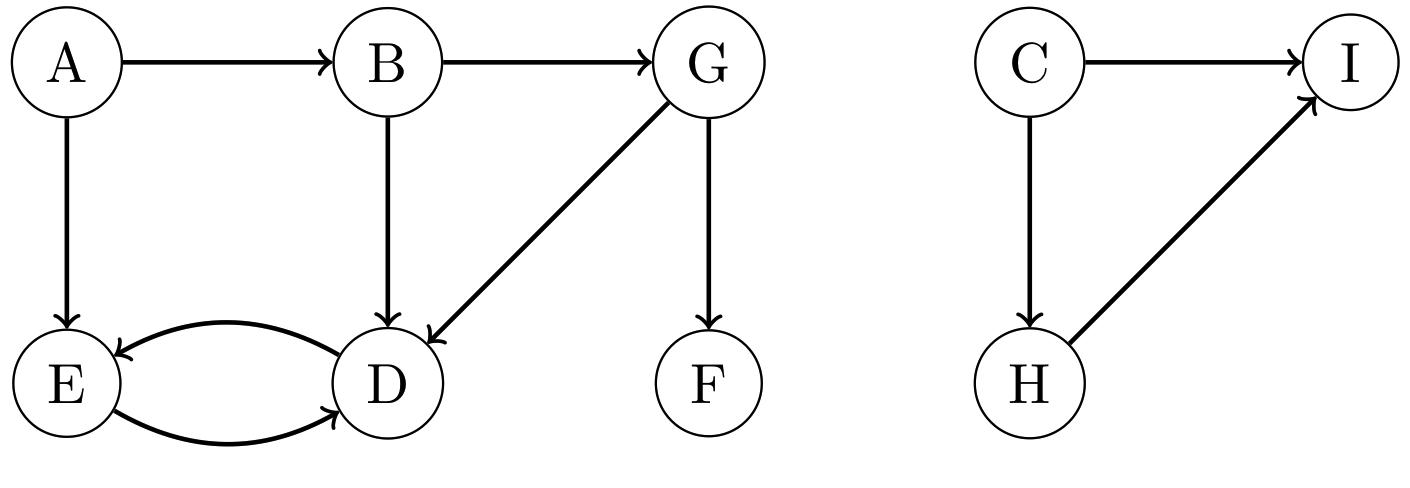
\includegraphics[width=6cm]{simple_graph.png} \\
  &\begin{tabular}{|c|c|c|c|c|c|c|c|c|c|}
    \hline
    A & B & D & E & E & D & G & F & F & G \\ \hline
    1 & 2 & 3 & 4 & 5 & 6 & 7 & 8 & 9 & 10 \\
    \hline
  \end{tabular}  \\
  &\begin{tabular}{|c|c|c|c|c|c|c|c|}
    \hline
    B & A & C & H & I & I & H & C \\ \hline
    11 & 12 & 13 & 14 & 15 & 16 & 17 & 18 \\
    \hline
  \end{tabular}   
    \end{align*}
    The pre- and post- numbers of a vertex refer to the time it was put on the stack and taken off the stack, respectively. So in the enumerated list above, $pre(v)$ and $post(v)$ are the times $v$ first appears and last appears, respectively. The edge types can be read off the pre- and post-numbers:
    \begin{align*}
    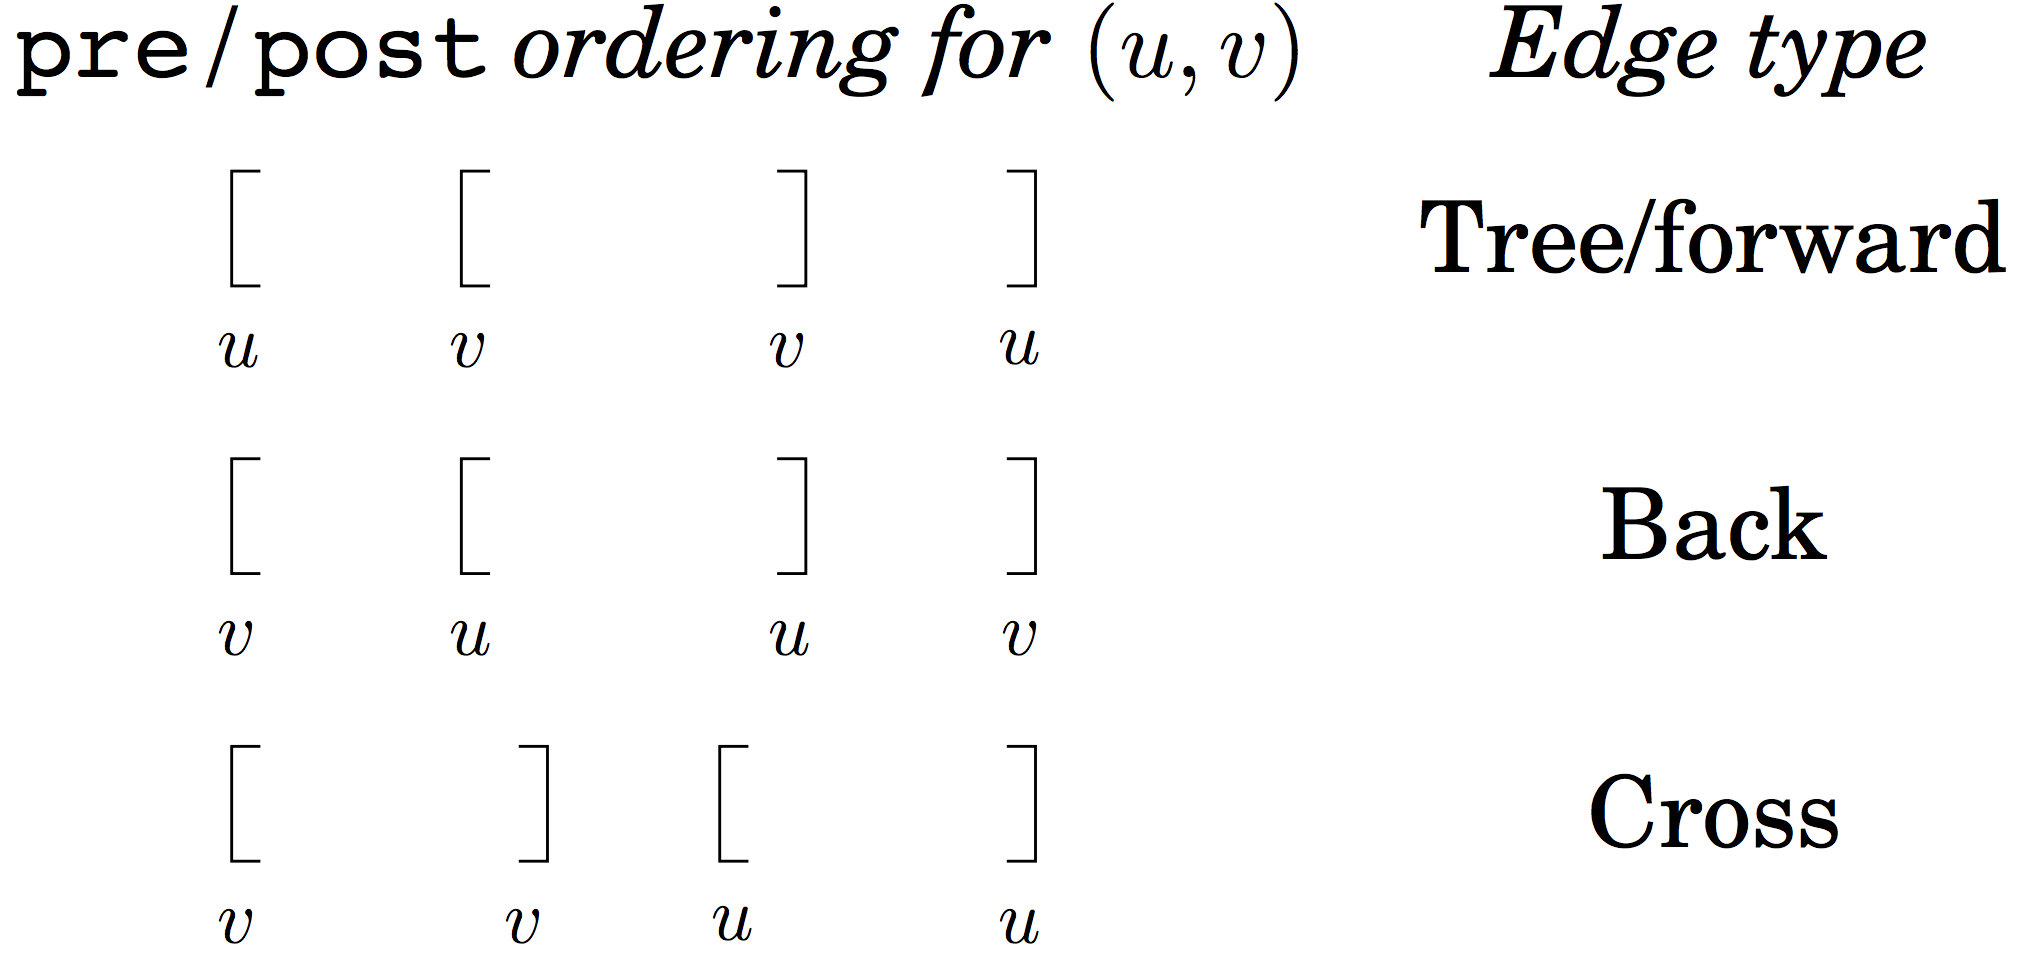
\includegraphics[width=6.5cm]{edge_types.png}
    \end{align*}
    where a tree edge is a direct edge actually used in the DFS procedure. A directed graph has a cycle iff its depth first search reveals a back edge. 
    
    \end{enumerate}
    
    \subsection{Strongly Connected Components}
    \begin{enumerate}[label=(\alph*)]
    \item A linearization, or \textbf{topological ordering}, is possible iff a graph is a \textbf{directed acyclic graph (DAG)}. A valid topological sort is one such that each edge goes from an earlier vertex to a later vertex, so that all precedence constraints are satisfied. This can be accomplished in $O(|V| + |E|)$ time, using a modified DFS: for each node, start a DFS that terminates when it hits any node that has already been visited since the beginning of the topological sort. Before removing a node from the stack, prepend it to an ouput list. The contents of the list by the end will be a valid linearization.
    \item Two nodes $u$ and $v$ of a \textit{directed} graph are connected if there is a path from $u$ to $v$ \textit{and} a path from $v$ to $u$. This relation partitions $V$ into disjoint sets called \textbf{strongly connected components.}
    \item If we shrink each strongly connected component down to a single meta-node, and draw an edge from one meta-node to another if there is an edge between their respective components, then the resulting meta-graph must be a DAG. An example is given below:
    \begin{align*}
    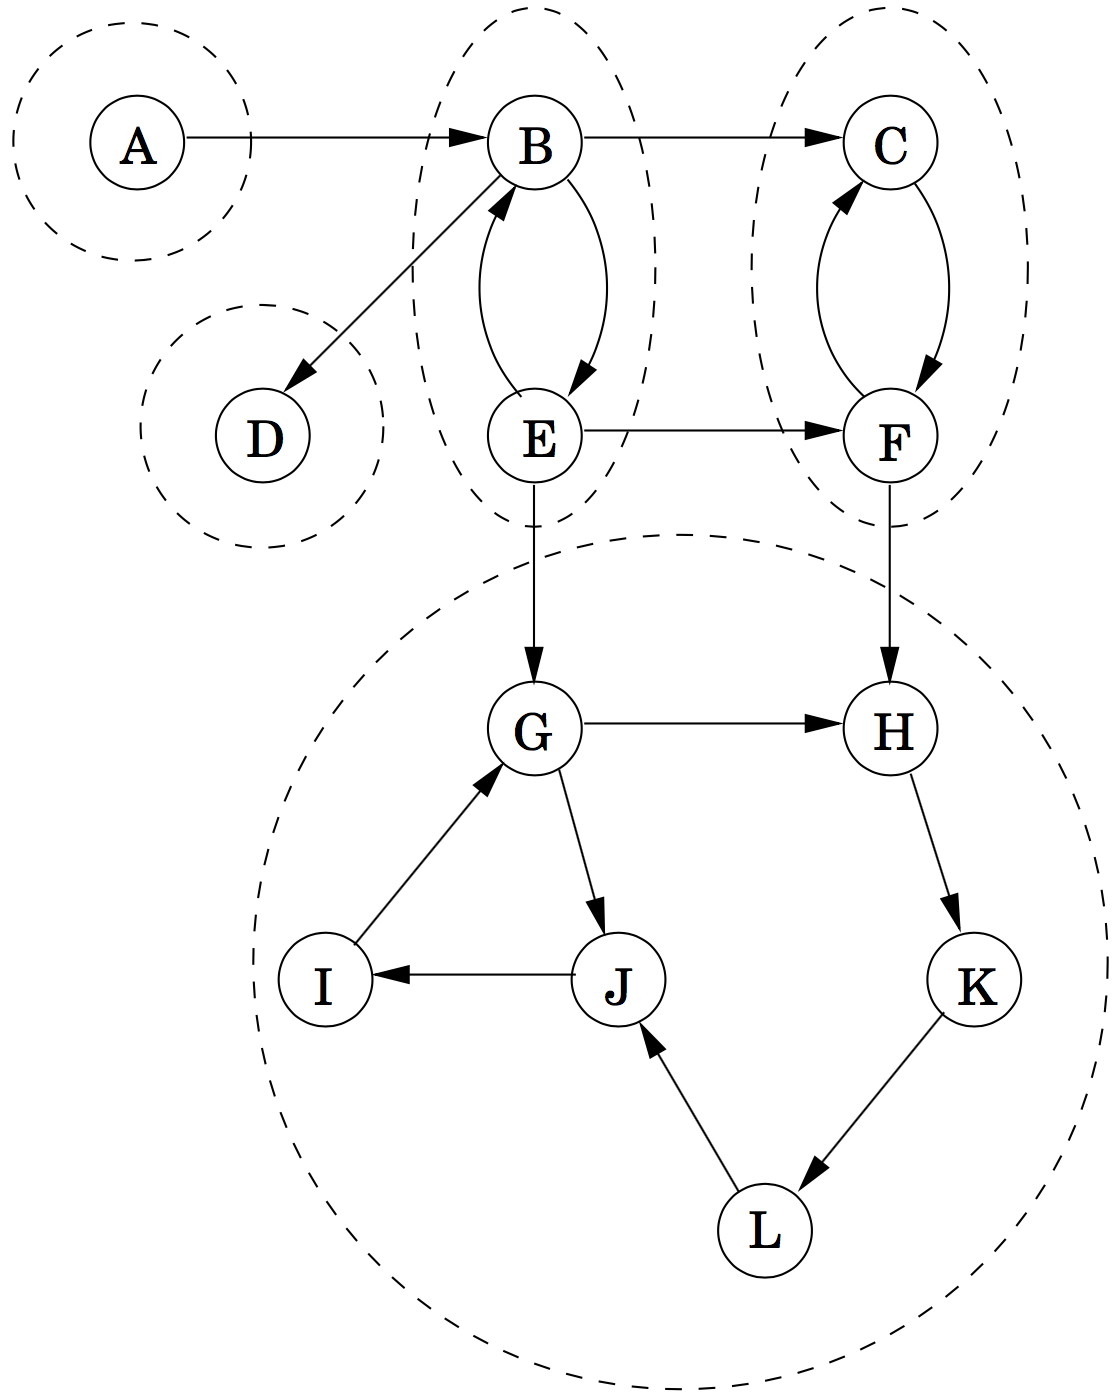
\includegraphics[width=4.6cm]{scc.png}
    \end{align*}
    \begin{align*}
        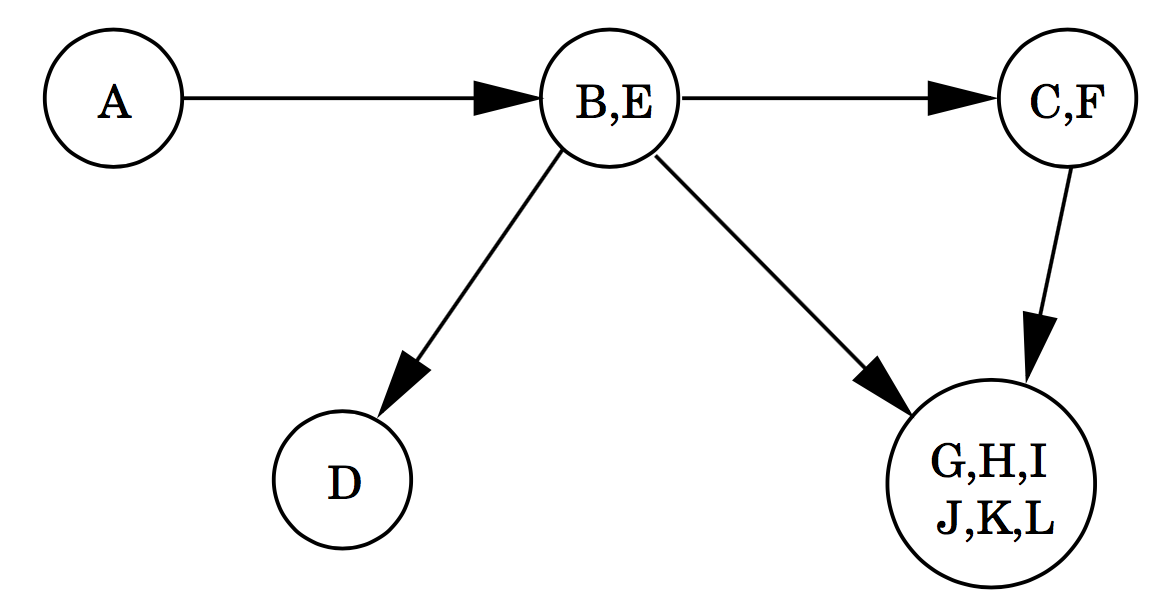
\includegraphics[width=4cm]{metanodes.png}
    \end{align*}
    
    \item A linear time $O(|V| + |E|)$ algorithm to output the strongly connected components of an undirected graph is possible.
    \item A key observation is that the node that receives the highest post number in a depth-first search must lie in a source strongly connected component.
    \item With this in mind, consider the reverse graph $G^R$, which is the same as $G$ except all edges are reversed. If we do a DFS of $G^R$, the node with the highest post number will come from a source strongly connected component in $G^R$, which is to say a sink strongly connected component in $G$.
    \item Observe that if the \texttt{explore} subroutine is started at node $u$, then it will terminate precisely when all nodes reachable from $u$ have been visited. Thus we can gather post-numbers from DFS on $G^R$, then run DFS on $G$ processing the vertices in decreasing order of their post numbers. Everytime \texttt{explore} terminates, output a strongly connected component and increment the component counter.
    \end{enumerate}
\end{addmargin}

\section{Paths in Graphs}
\begin{addmargin}[0.8em]{0.5em}
    \subsection{Breadth First Search}
    \begin{enumerate}[label=(\alph*)]
        \item Define the \textbf{distance} between two nodes as the length of the shortest path between them.
        \item For all vertices $u$ reachable from $s$, dist($u$) is set to the distance from $s$ to $u$:        
\begin{minted}[linenos=false, escapeinside=??, mathescape=true]{octave}
function BFS(?$G,s$?)
for all ?$u \in V$?:
    dist(?$u$?) = ?$\infty$?
dist(?$s$?) = 0
Q = ?$[s]$?
while not Q.isEmpty():
    ?$u$? = Q.pop()
    for all edges ?$(u, v) \in E$?:
        if dist(?$v$?) = ?$\infty$?:
            Q.enqueue(?$v$?)
            dist(?$v$?) = dist(?$u$?) + 1
\end{minted}
        Like DFS, BFS has linear runtime $O(|V| + |E|)$. Notice the code is almost identical to DFS but with a queue in place of a stack; this results in a broader, shallower search. Note that in this implementation, we do not restart the search in other connected components.

    \end{enumerate}
    
    \subsection{Dijkstra’s algorithm}
    \begin{enumerate}[label=(\alph*)]
        \item Now we consider each edge $e$ from $u$ to $v$ being annotated with length $l(u,v)$. For now, we must have positive edge lengths.
\begin{minted}[linenos=false, escapeinside=??, mathescape=true]{octave}
function Dijkstra(?$G,s$?)
for all ?$u \in V$?:
    dist(?$u$?) = ?$\infty$?
    prev(?$u$?) = null
dist(?$s$?) = 0
H = makeQueue(?$V$?)
while not H.isEmpty():
    ?$u$? = H.deleteMin()
    for all edges ?$(u,v) \in E$?:
        if dist(?$v$?) > dist(?$u$?) + ?$l(u,v)$?:
            dist(?$v$?) = dist(?$u$?) + ?$l(u,v)$?
            prev(?$v$?) = ?$u$?
            H.decreaseKey(?$v$?)
\end{minted}
\item Dijkstra’s algorithm is essentially just BFS, except it uses a priority queue so as to prioritize nodes in a way that takes edge lengths into account.
\item The running time of Dijkstra’s algorithm depends on the implementation of the priority queue. There are $|V|$ \texttt{deleteMin} operations and $|V| + |E|$ \texttt{insert} / \texttt{decreaseKey} operations. Using a $d$-ary heap (generalization of a binary heap), this yields a runtime of $O((|V| \cdot d + |E|) \frac{\log{|V|}}{\log{d}})$. The optimal choice is $d \approx \frac{|E|}{|V|}$, i.e., the average degree of the graph. A Fibonacci heap is a sophisticated data structure with a constant amortized cost for \texttt{insert} or \texttt{decreaseKey}, yielding a runtime of $O(|E| + |V|\log{|V|})$. 
    \end{enumerate}
    \subsection{Bellman Ford}
    \begin{enumerate}[label=(\alph*)]
        \item Dijkstra’s algorithm fails for graphs with negative edge weights. The Bellman-Ford algorithm, which has runtime $O(|V| \cdot |E|)$ is slower, but can handle this case.
\begin{minted}[linenos=false, escapeinside=??, mathescape=true]{octave}
function BellmanFord(?$G,s$?)
for all ?$u \in V$?:
    dist(?$u$?) = ?$\infty$?
    prev(?$u$?) = null
dist(?$s$?) = 0
repeat ?$|V| - 1$? times:
    for all ?$e \in E$?:
        update(?$e$?)
            
function update(?$(u,v)\in E$?)
dist(?$v$?) = min(dist(?$v$?), dist(?$u$?) + ?$l(u,v)$?)
\end{minted}
\item In implementation, we can have an extra check to make the loop terminate immediately after any round in which no update occurred.
\item If $G$ contains negative cycles, it doesn't make sense to talk about shortest paths. Bellman-Ford can easily detect such cycles: instead of stopping after $|V| - 1$ iterations, perform one extra round. There is a negative cycle iff some \texttt{dist} value is reduced during this final round.

\item If $G$ is a DAG, a linear time ($O(|V| + |E|)$) shortest paths algorithm is possible. The key point is that \textit{in any path of a DAG, the vertices appear in increasing linearized order.} 
\begin{minted}[linenos=false, escapeinside=??, mathescape=true]{octave}
function DAGShortestPaths(?$G,s$?)
for all ?$u \in V$?:
    dist(?$u$?) = ?$\infty$?
    prev(?$u$?) = null
dist(?$s$?) = 0
G.linearize()
for each ?$u \in V$?: # in linearized order
    for all edges ?$(u,v)\in E$?:
        update(?$(u,v)$?)
\end{minted}

    We can find the longest paths in a DAG by the same algorithm: just negate all edge lengths. As we will see later, this is an example of a simple dynamic programming problem.
 
    \end{enumerate}
\end{addmargin}

\section{Greedy Algorithms}
\begin{addmargin}[0.8em]{0.5em}
Greedy algorithms build up a solution piece by piece, always choosing the next piece that offers the most obvious and immediate benefit. Although this fails for most cases, there are some tasks for which it is optimal.
    \subsection{Minimum Spanning Trees}
    \begin{enumerate}[label=(\alph*)]
        \item A minimum spanning tree (MST) is a subset of the edges of a connected, edge-weighted undirected graph that connects all the vertices together with the minimum possible total edge weight.
        \item A tree is an undirected graph that is connected and acyclic. Some properties:
        \begin{enumerate}[label=(\roman*)]
        \item A tree on $n$ nodes has $n - 1$ edges.
        \item Any connected, undirected graph $G = (V, E)$ with $|E| = |V | - 1$ is a tree.
        \item An undirected graph is a tree if and only if there is a unique path between any pair of nodes.
        \end{enumerate}
        \item A \textit{cut} is any partition of vertices into two groups, $S$ and $V - S$. The \textit{cut property} tells us how to choose the next edge in building a MST: suppose edges $X$ are part of a minimum spanning tree of $G$. Pick any subset of nodes $S$ for which $X$ does not cross between $S$ and $V - S$, and let $e$ be the lightest edge across this partition. Then $X \cup \{e\}$ is part of some MST.
        \item \textbf{Kruskal’s MST algorithm:}
\begin{minted}[linenos=false, escapeinside=??, mathescape=true]{octave}
function kruskal(?$G$?)
for all ?$u \in V$?:
    makeset(?$u$?)
?$X = \{ \}$?
Sort edges ?$E$? by weight
for all edges ?$\{u,v\} \in E$?: # ordered by weight
    if find(?$u$?) ?$\neq$? find(?$v$?):
        add edge ?$\{u,v\}$? to ?$X$?
        union?$(u,v)$?
\end{minted}
        The output MST is defined by the edges $X$. Here make use of the disjoint set data structure. \texttt{makeset}($x$) creates a set containing just $x$. \texttt{find}($x$) returns the set to which $x$ belongs. \texttt{union}($x, y$) merges the sets containing $x$ and $y$.
        \item An efficient data structure for disjoint sets involves storing the sets as upward directed trees with all nodes eventually leading up to the root (which has a natural implementation as an array):
\begin{minted}[linenos=false, escapeinside=??, mathescape=true]{octave}
function makeset(?$x$?)
?$\pi(x) = x$?
rank?$(x) = 0$?

function find(?$x$?)
while ?$x \neq \pi(x): \hspace{5pt} x = \pi(x)$?
return ?$x$?

function union(?$x,y$?)
?$r_x$?, ?$r_y$? = find(?$x$?), find(?$y$?)
if ?$r_x = r_y$?: return
if rank?$(r_x)$? > rank?$(r_y)$?: ?$\pi(r_y) = r_x$?
else: ?$\pi(r_x) = r_y$?
if rank?$(r_x)$? = rank?$(r_y)$?: rank?$(r_y)$? += 1
\end{minted}      
        where $\pi(x)$ denotes the parent of $x$ and \texttt{rank}($x$) represents the height of the subtree rooted at $x$. All the trees have height $\leq \log{n}$, so that \texttt{makeset} is $O(1)$, \texttt{find} is $O(\log{n})$, and \texttt{union} is $O(\log{n})$.
        \item With this data structure, the total time for Kruskal’s algorithm becomes $O(|E| \log{|V|})$ for sorting the edges (since $\log{|E|} \approx \log{|V|}$) plus another $O(|E| \log{|V|})$ for the \texttt{union} and \texttt{find} operations.
        \item Using path compression, the amortized cost for \texttt{find} turns out to be very nearly $O(1)$:
\begin{minted}[linenos=false, escapeinside=??, mathescape=true]{octave}
function find(?$x$?)
if ?$x \neq \pi(x): \hspace{5pt} \pi(x) = $? find?$(\pi(x))$?
return ?$\pi(x)$?
\end{minted}        
        \item Another MST algorithm is a variant of Dijkstra's, where the priority queue is ordered by the weight of the lightest incoming edge from set $S$, instead of the length of an entire path to that node from the starting point. It has the same running time as Dijkstra's.
        \item \textbf{Prim's MST algorithm}:
\begin{minted}[linenos=false, escapeinside=??, mathescape=true]{octave}
function prim(?$G$?)
for all ?$u \in V$?:
    cost(?$u$?) = ?$\infty$?
    prev(?$u$?) = null
pick initial node ?$u_0$?
cost(?$u_0$?) = 0
H = makeQueue(?$V$?)
while not H.isEmpty():
    ?$v$? = H.deleteMin()
    for each ?$\{v,z\} \in E$?:
        if cost(?$z$?) > ?$l(v,z)$?:
            cost(?$z$?) = ?$l(v,z)$?
            prev(?$z$?) = ?$v$?
            H.decreaseKey(?$z$?)
\end{minted}
        The output MST is defined by the array \texttt{prev}.
    \end{enumerate}
    
    \subsection{Huffman encoding}
    \begin{enumerate}[label=(\alph*)]
        \item Huffman coding is a form of lossless data compression. The idea is to optimally encode an alphabet using \textit{variable-length encoding}, where the lengths of the assigned codes (bit sequences) are based on the frequencies of the characters; the most frequent character gets the shortest code and the least frequent character gets the longest code.
        \item The codes are prefix-free, meaning they are assigned in such a way that no codeword can be a prefix of another codeword, so as to prevent ambiguity when decoding a bit stream.
        \item The first step is to build the Huffman tree, a full binary tree with $2n-1$ nodes, where the codewords are at the leaves:
\begin{minted}[linenos=false, escapeinside=??, mathescape=true]{octave}
function Huffman(?$f[1,\hdots,n]$?) 
let H be priority queue ordered by ?$f$?
for ?$i=1$? to ?$n$?: H.insert(?$i$?)
for ?$k=n+1$? to ?$2n-1$?:
    ?$i$?, ?$j$? = H.deleteMin(), H.deleteMin()
    create node ?$k$? with children ?$i,j$?
    ?$f[k] = f[i] + f[j]$?
    H.insert(?$k$?)
\end{minted}
    Here we create a leaf node for each character, then iteratively create the internal nodes from the bottom up. In the example below, the frequencies are in brackets:
    \begin{align*}
    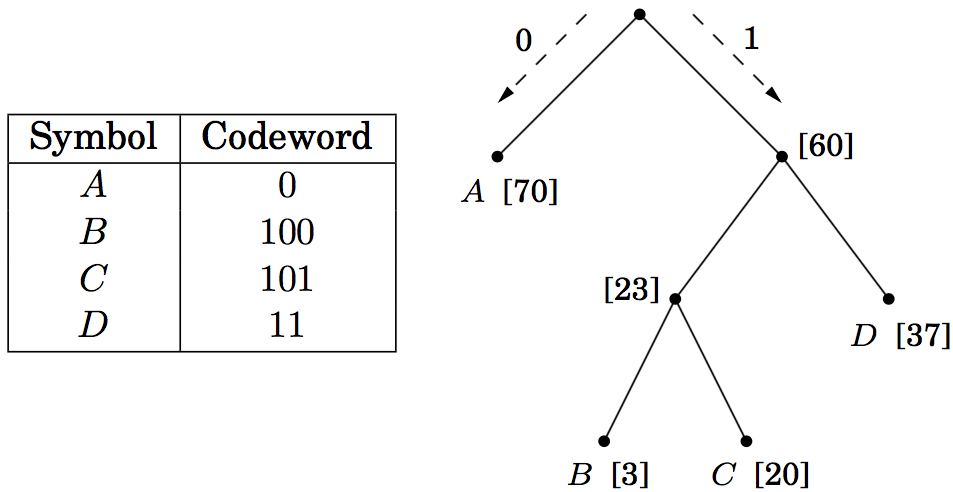
\includegraphics[height=3.8cm]{huffman.png}
    \end{align*}
    \item Decoding is done by repeatedly starting at the root, reading the stream to move downward until a leaf is reached, and outputting the corresponding symbol.
    \end{enumerate}
    
    \subsection{Horn-satisfiability}
    \begin{enumerate}[label=(\alph*)]
        \item There are two types of Horn clauses: implication, whose left-hand side is an AND of  positive literals and whose right-hand side is a single positive literal (a literal is a boolean variable or its negation); and pure negative clauses consisting of an OR of negative literals.
        \item HornSAT is the problem of finding is a given set of propositional Horn clauses is satisfiable; that is, there is an assignment of true/false values to the variables that satisfies all the clauses. The algorithm can be implemented with running time linear in the number of clauses.
        \item The algorithm is as follows: set all variables to false. While there is an implication that is not satisfied, set the right-hand variable of the implication to true. If all pure negative clauses are satisfied, return the assignment. Otherwise, the formula is not satisfiable.
        \item The algorithm is correct because of the following invariant: if a certain set of variables is set to true, then they must be true in any satisfying assignment. Hence, if the truth assignment found after the while loop does not satisfy the negative clauses, there can be no satisfying truth assignment.
    \end{enumerate}
    
    \subsection{Set Cover}
    \begin{enumerate}[label=(\alph*)]
        \item A set cover problem is of the following form: Given a set $B$, and $S_1, \hdots, S_m \subseteq B$, find a selection of the $S_i$ whose union is $B$, using the fewest number of sets.
        \item A greedy solution is as follows: While the elements of $B$ are uncovered, pick the set $S_i$ with the largest number of uncovered elements.
        \item This solution is not optimal, but is close to optimal: if $B$ contains $n$ elements and the optimal cover consists of $k$ sets, then the Greedy algorithm will use at most $k \ln{n}$ sets.
        \item To see this, let $n_t$ denote the number of elements still not covered after $t$ iterations of the greedy algorithm (so $n_0 = n$). Since these remaining elements are covered by the optimal $k$ sets, there must be some set with at least $n_t/k$ of them. Therefore, the greedy strategy will ensure that 
        $$
        n_{t+1} \leq n_t - \frac{n_t}{k} = n_t \left( 1 - \frac{1}{k} \right)
        $$
        Iterating this, we have $n_t \leq n_0 (1 - 1/k)^t$. Now using the inequality $1-x \leq e^{-x}$, with equality iff $x=0$, we have
        $$
        n_t \leq n_0 \left(1 - \frac{1}{k} \right)^t < n_0 (e^{-1/k})^t = ne^{-t/k}
        $$
        At $t=k\ln{n}$, $n_t$ is less than $ne^{-\ln{n}}=1$, which means no elements remain to be covered.
        \item The maximum ratio between the greedy algorithm’s solution and the optimal solution is called the \textit{approximation factor}. There is provably no polynomial-time algorithm with a smaller approximation factor for set cover.
    \end{enumerate}
    
    \subsection{Task Scheduling}
    \begin{enumerate}[label=(\alph*)]
        \item We have a set of $n$ tasks, each represented by an interval $(s_i, f_i)$ for start and finish time $s_i$, $f_i$, respectively. The goal is to find the maximum subset of mutually compatible tasks, so that we can schedule as many tasks as possible.
        \item Several greedy strategies that may seem promising actually do not find the optimal solution. Counterexamples to some incorrect approaches are shown below (green denotes the next task to be selected by the strategy):
        \begin{center}
        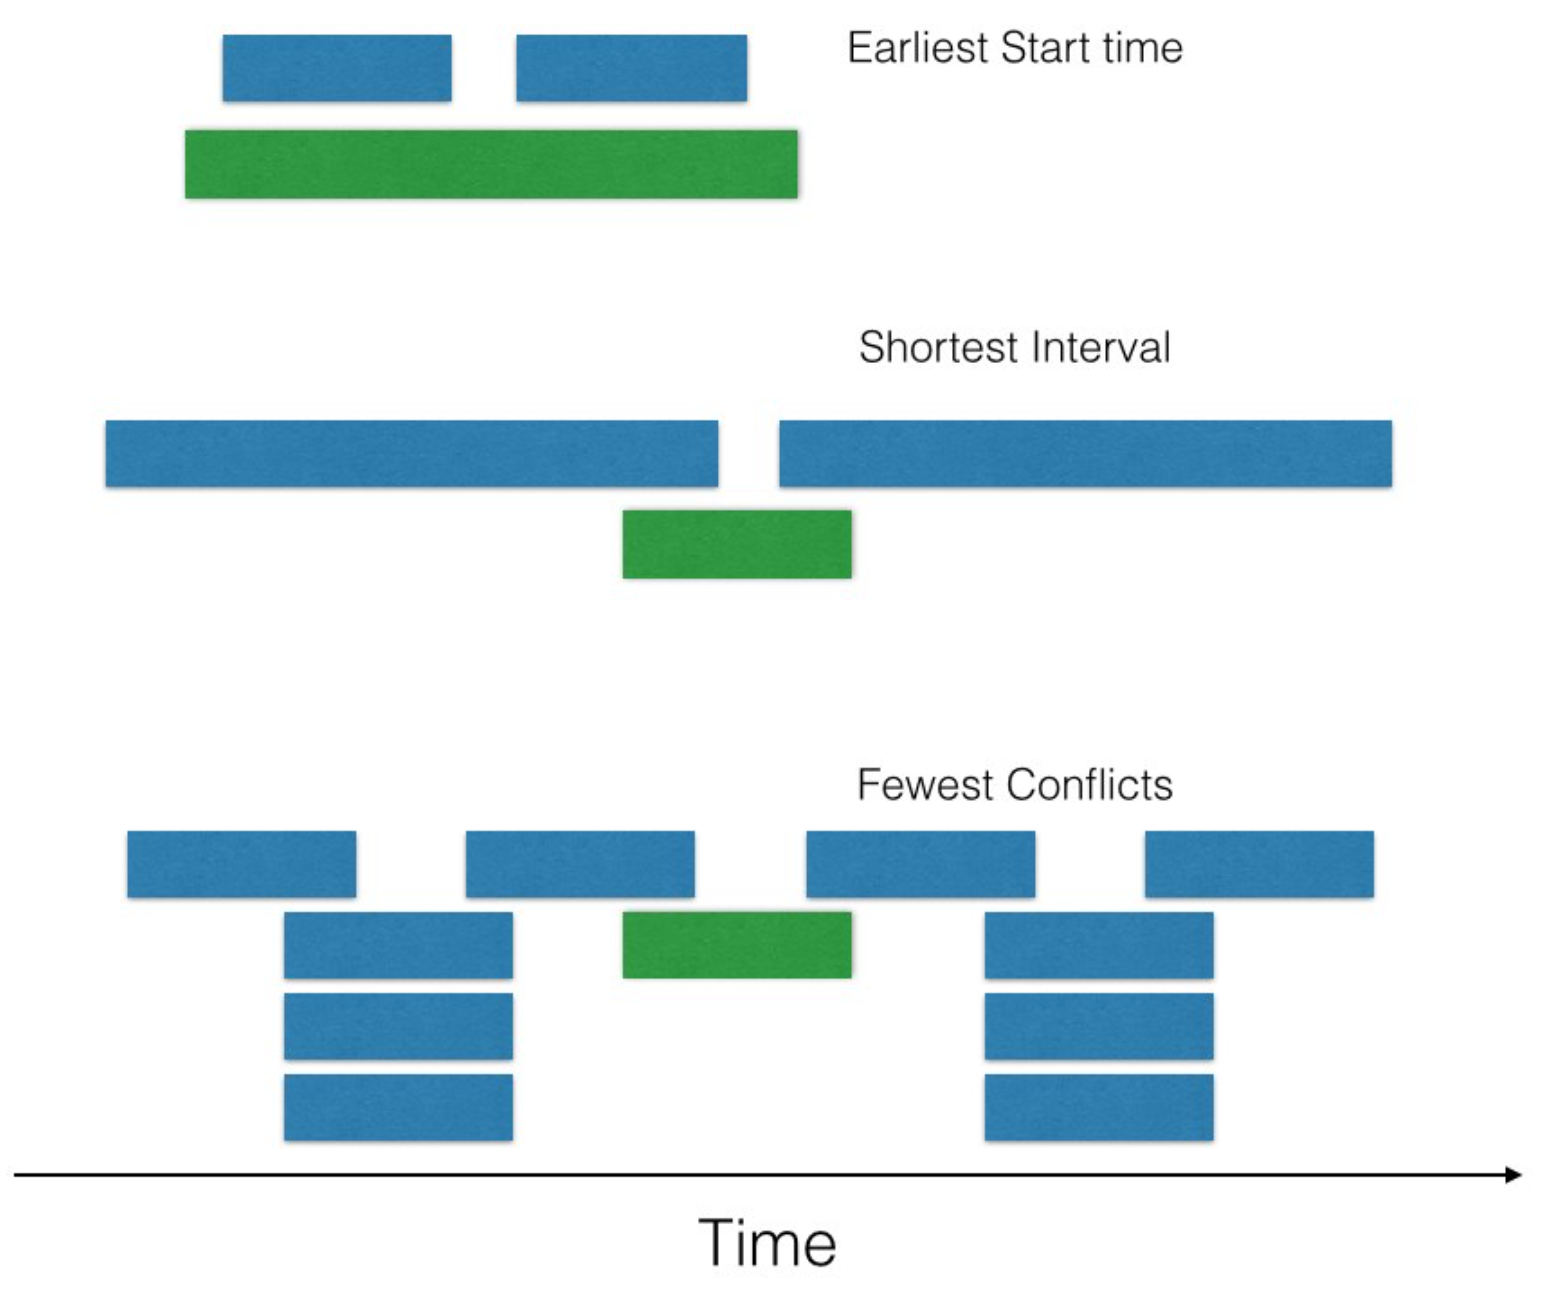
\includegraphics[width=5cm]{scheduling.png}
        \end{center}
        \item The following greedy strategy \textit{does} find the optimal solution: consider tasks in ascending order of $f_i$; that is, by earliest finish time. (1) Find the task $t$ with earliest finish time; (2) remove said task $t$, and all intervals intersecting $t$, from the set of candidate tasks. Repeat until no tasks remain.
        \item The reasoning is as follows: whenever we select a task $t$ in step (1), we may have to remove many intervals in step (2). However, all these intervals necessarily cross the finishing time of $t$, and thus they all cross each other. Hence, at most 1 of these intervals can be in the optimal solution. Choosing the first task to be finished among these intersecting intervals guarantees the greatest ``availability" for future tasks.
    \end{enumerate}
\end{addmargin}

\section{Dynamic Programming}
\begin{addmargin}[0.8em]{0.5em}
Dynamic programming is an algorithmic paradigm in which a complex problem is solved by breaking it down into a collection of simpler subproblems, solving each of those subproblems just once, and storing their solutions.
    \subsection{Longest Increasing Subsequence}
    \vspace{-0.2cm}
    \begin{enumerate}[label=(\alph*)]
        \item Given a sequence of numbers $a_1, \hdots, a_n$, a \textit{subsequence} is any subset of these numbers taken in order, and an \textit{increasing} subsequence is one in which the numbers are getting strictly larger. The task is to find the increasing subsequence of greatest length.
        \item There is an implicit DAG in all dynamic programming problems: the nodes are the subproblems we define, and the edges are the dependencies between the subproblems. 
        \item In this problem, we establish a node $i$ for each element $a_i$, and add directed edges $(i, j)$ whenever it is possible for $a_i$ and $a_j$ to be consecutive elements in an increasing subsequence. 
        % For example:
        % \begin{align*}
        % 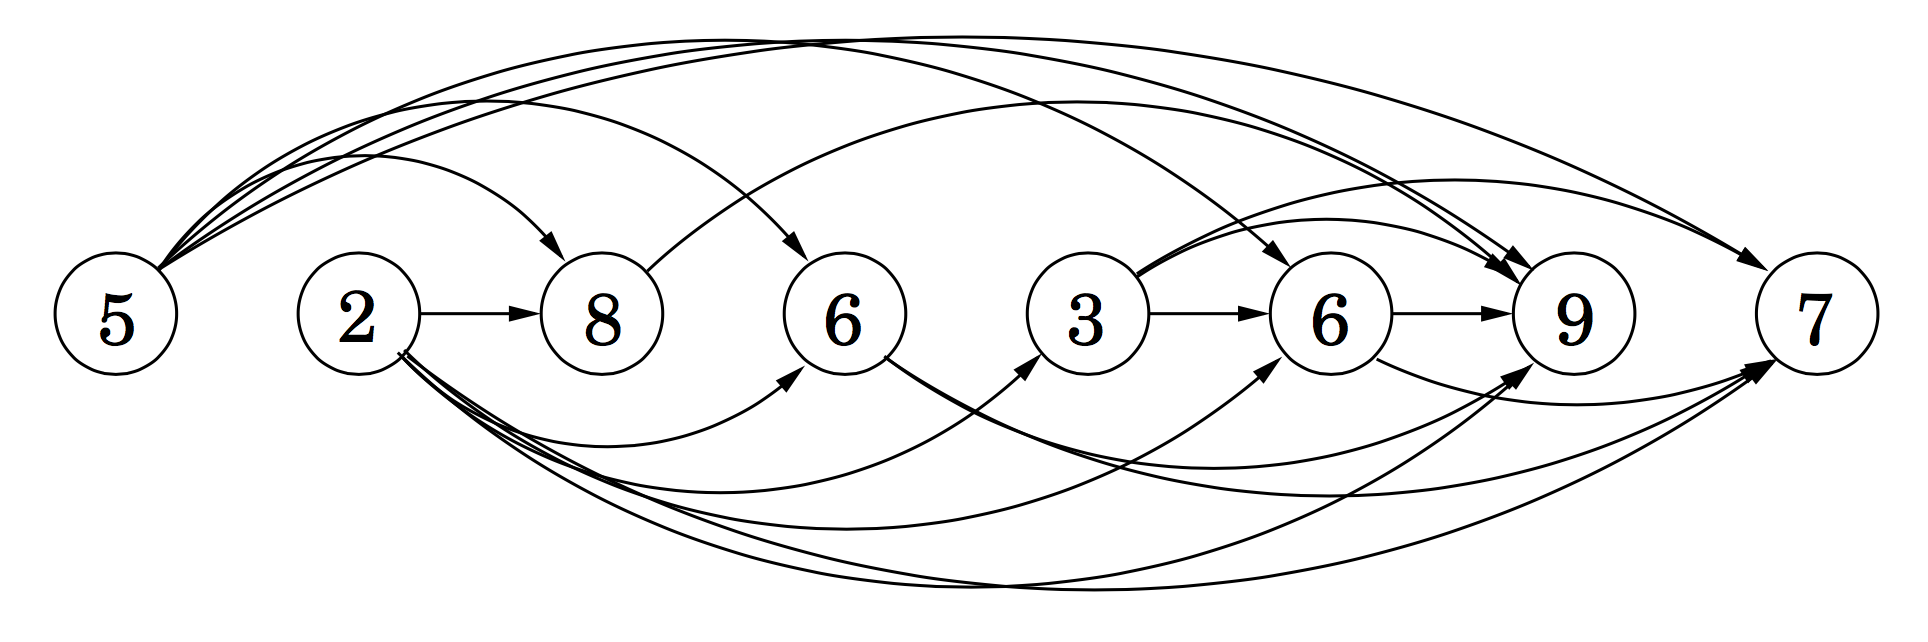
\includegraphics[width=5.5cm]{dp_dag.png}
        % \end{align*}
        The solution is simply the longest path in the DAG:
        \begin{minted}[linenos=false, escapeinside=??, mathescape=true]{octave}
function longestIncreasingSubseq(?$[a_1, \hdots, a_n]$?)
for ?$j=1, \hdots, n$?:
    ?$L(j)$? = 1 + max{?$L(i) : (i,j) \in E$?}
return max?$_{j} L(j)$?
        \end{minted}
        where $L(j)$ represents the length of the longest path (i.e. longest increasing subsequence) ending at $j$. The overall running time is $O(|E|)$, which is at most $O(n^2)$ when the input array is sorted.
        
        \item To actually recover the longest subsequence, we should store back pointers when an entry is set - this will be a common theme throughout dynamic programming, and will be assumed from now on.
    \end{enumerate}        
        
    \subsection{Edit distance}
    \vspace{-0.2cm}
    \begin{enumerate}[label=(\alph*)]
        \item Given two strings, the edit distance is the minimum cost (number of indices where characters differ) of all possible alignments of the two strings.
        \begin{align*}
        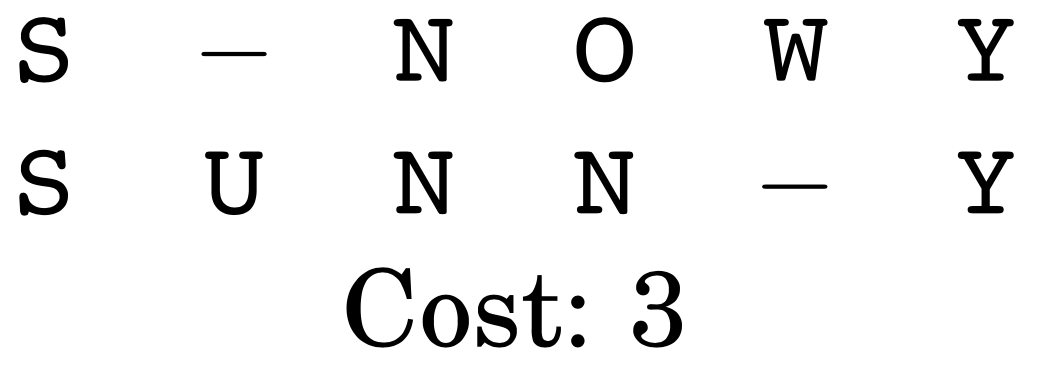
\includegraphics[width=3cm]{str_align.png}
        \end{align*}
        The best possible alignment of \texttt{SNOWY} and \texttt{SUNNY} is given above, so the edit distance is 3. It is so named because it is the minimum number of edits (insertions, deletions, or substitutions of characters) needed to transform the first string into the second.
        
        \item Suppose we have strings $x[1 \cdots m]$ and $y[1 \cdots n]$. Define $E(i,j)$ to be the edit distance between $x[1 \cdots i]$ and $y[1 \cdots j]$. The rightmost column of the best alignment between $x[1 \cdots i]$ and $y[1 \cdots j]$ can be one of three things:
        \begin{align*}
        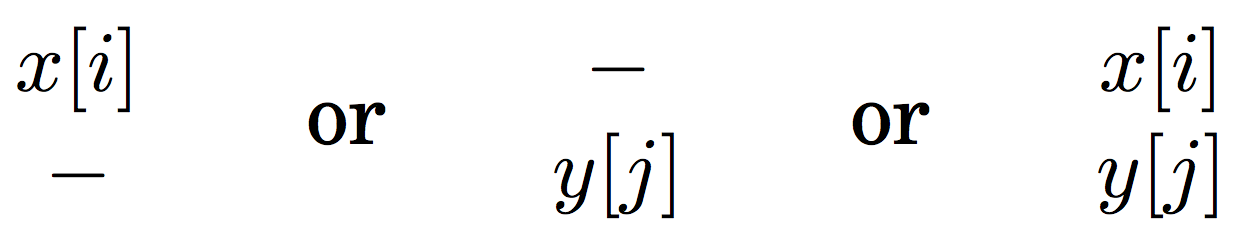
\includegraphics[width=4cm]{edalign.png}
        \end{align*}
        The first two cases have a cost of $1 + E(i-1, j)$ and $1 + E(i, j-1)$, respectively. The final case has cost $1$ (if $x[i] \neq y[j]$) or $0$ (if $x[i] = y[j]$), plus $E(i-1, j-1)$.
        \item The subproblems naturally form a $m \times n$ grid, where the goal $E(m,n)$ is the last entry. Any order of populating the grid is fine, as long as $E(i - 1, j)$, $E(i, j - 1)$, and $E(i - 1, j - 1)$ are handled before $E(i, j)$. Going row by row, from left to right:
        \begin{minted}[linenos=false, escapeinside=??, mathescape=true]{octave}
function editDistance(?$x[1 \cdots m], y[1 \cdots n]$?)
for ?$i=0, 1, \hdots, m$?:
    ?$E(i,0) = i$?
for ?$j=1, \hdots, n$?:
    ?$E(0,j) = j$?
for ?$i=1, \hdots, m$?:
    for ?$j=1, \hdots, n$?:
        c1 = ?$E(i-1,j)+1$?
        c2 = ?$E(i,j-1)+1$?
        c3 = ?$E(i-1,j-1) + \text{diff}(i,j)$?
        ?$E(i,j)$? = min{c1, c2, c3}
return ?$E(m,n)$?        
        \end{minted}
        The running time is $O(mn)$. 
        % \item The underlying DAG has the form
        % \begin{align*}
        % 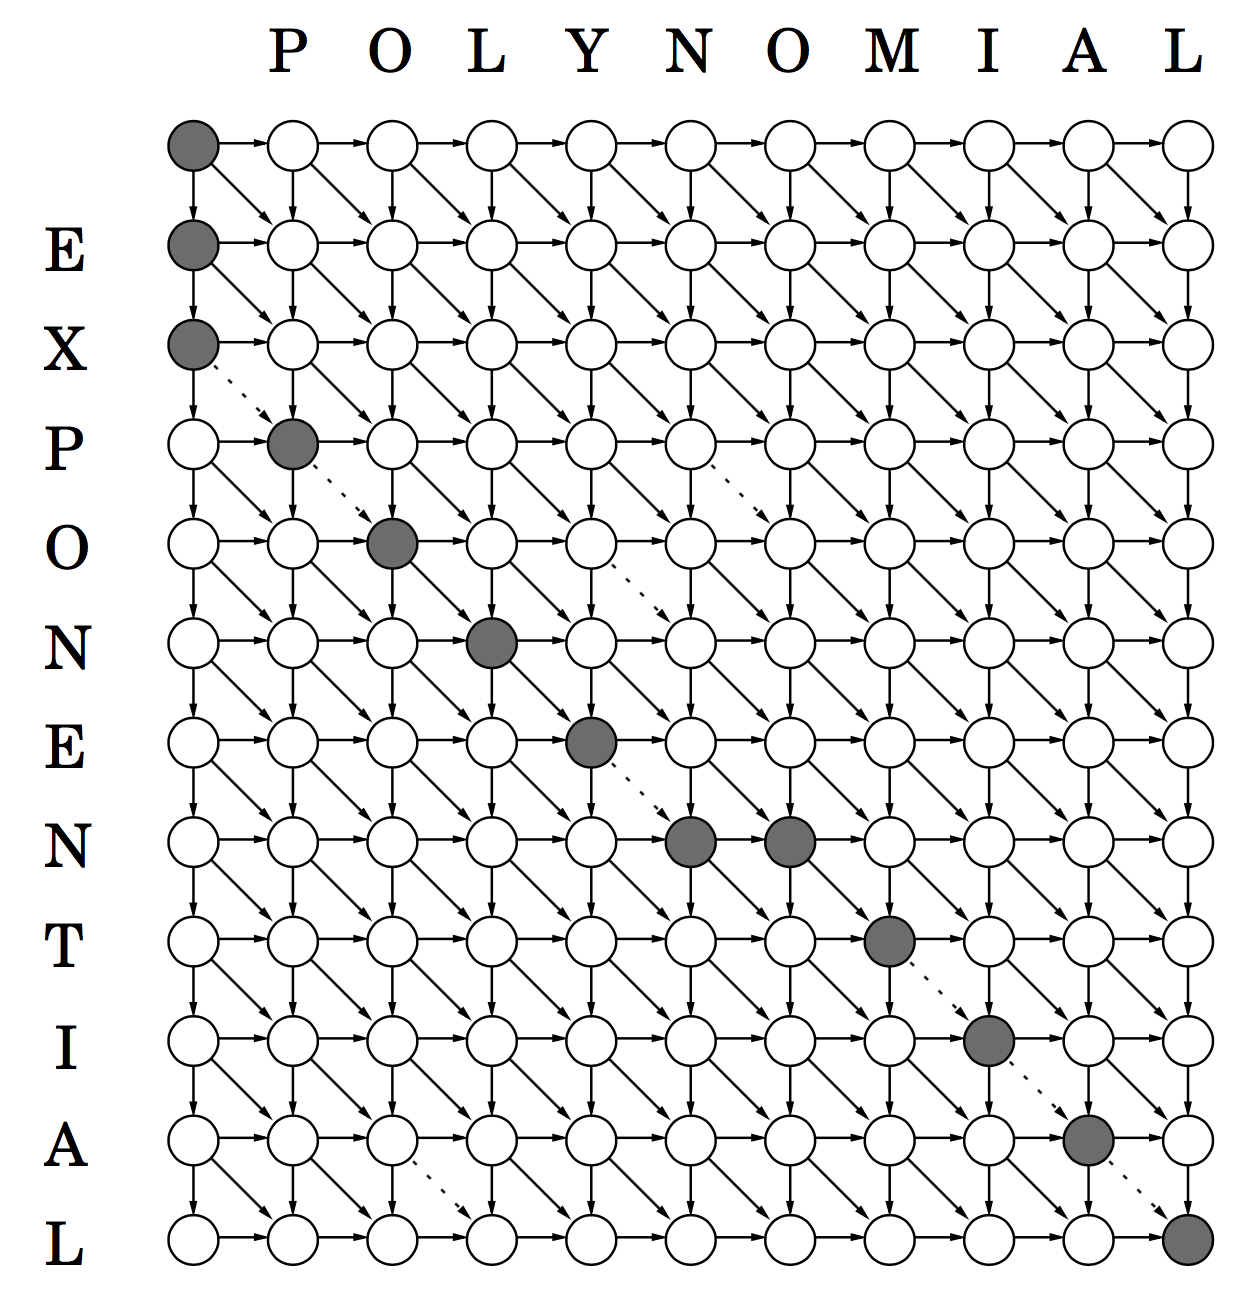
\includegraphics[width=4.4cm]{edit_dag.png}
        % \end{align*}
        % Set all edge weights to 1, except for edges $(i-1,j-1) \to (i,j), x[i]=y[j]$ (shown dotted), which we set to 0. The edit distance is then given by the shortest path in the DAG. Each down move is a deletion, each right move is an insertion, and each diagonal move is either a match or a substitution. By altering the weights on this dag, we can give insertions, deletions, and substitutions different associated costs.
        % \item Dynamic programming lies at the heart of nearly all DNA sequencing problems that make up the field of computational biology.
    \end{enumerate}        
        
    \subsection{Knapsack}
    \begin{enumerate}[label=(\alph*)]
        \item The knapsack problem generalizes a wide variety of resource-constrained selection tasks. Given a set of $n$ items, each with a weight $w_i$ and a value $v_i$, the task is to determine the most valuable combination of items with total weight less than or equal to a given limit $W$.
        \item First we consider knapsack with repetition of items allowed. Define $K(w)$ to be the maximum value achievable with a knapsack of capacity $w$. If the optimal solution to $K(w)$ includes item $i$, then removing this item from the knapsack leaves an optimal solution to $K(w - w_i)$ for some $i$. We need to try all possibilities of $i$:
        $$
        K(w) = \max_{i: w_i \leq w} \{ K(w - w_i) + v_i \}
        $$
        This leads to the following algorithm:
        \begin{minted}[linenos=false, escapeinside=??, mathescape=true]{octave}
function knapsack1(?$w[1 \cdots n], v[1 \cdots n], W$?)
?$K(0) = 0$?
for ?$w=1$? to ?$W$?:
    ?$K(w)$? = max{?$K(w-w_i)+v_i \mid w_i \leq w$?}
return ?$K(W)$?
        \end{minted}
        The overall running time is $O(nW)$, since each entry in the array takes up to $O(n)$ time to compute.
        
        \item Knapsack without repetition requires a second parameter about the items already used. Define $K(w,j)$ to be the maximum value achievable using a knapsack of capacity $w$ and items $1,\hdots,j$. There are two cases: either item $j$ is needed to achieve the optimal value, or it isn't:
        $$
        K(w,j) = \max\{ K(w-w_j, j-1) + v_j, K(w, j-1) \}
        $$
        This leads to the following algorithm:
        \begin{minted}[linenos=false, escapeinside=??, mathescape=true]{octave}
function knapsack2(?$w[1 \cdots n], v[1 \cdots n], W$?)
?$\forall j: K(0,j)=0$?, ?$\forall w: K(w,0)=0$?
for ?$j=1$? to ?$n$?:
    for ?$w=1$? to ?$W$?:
        c1 = ?$K(w-w_j, j-1)+v_j$?
        c2 = ?$K(w, j-1)$?
        if ?$w_j > w$?: ?$K(w,j)$? = c2
        else: ?$K(w,j)$? = max{c1, c2}
return ?$K(W,n)$?
        \end{minted}
        The overall running time is still $O(nW)$, since each entry in the grid takes constant time to compute.
        \item We say the Knapsack algorithm's run-time is \textit{pseudopolynomial}: it depends on the magnitude of the $W$, which is exponential in how it is represented in binary $(2^n)$.
        
        \item In dynamic programming, we write out a recursive formula that expresses large problems in terms of smaller ones and then use it to fill out a table of solution values in a bottom-up manner. We could also use recursion with \textit{memoization}: storing the values of a function call in a hashmap. The constant factor is substantially larger because of the overhead of recursion. However, memoization can pay off in some cases because memoization only ends up solving the subproblems that are actually used.
    \end{enumerate}    
    \vspace{-0.4cm}
    \subsection{Chain matrix multiplication}
    \vspace{-0.2cm}
    \begin{enumerate}[label=(\alph*)]
        \item Computing the product of a chain of matrices involves iteratively multiplying two matrices at a time. Multiplying a $m \times n$ matrix by a $n \times p$ matrix takes about $mnp$ multiplications. The order in which the matrices are grouped in the multiplication makes a big difference in the final running time.
        \item Consider the product $A_1A_2 \cdots A_n$ where each $A_i$ is a matrix of dimension $m_{i-1} \times m_i$. For $1 \leq i \leq j \leq n$, define $C(i,j)$ to be the minimum cost of multiplying $A_iA_{i+1} \cdots A_j$. We break the product into $A_iA_{i+1} \cdots A_k$ and $A_{k+1}A_{k+2} \cdots A_j$ for some $k$ between $i$ and $j$. The cost is then the cost of these two partial products, and the cost of combining them:
        \begin{align*}
        C(i,j) = \min_{i \leq k < j} \{ C(i,k) + C(k+1,j) + m_{i-1} m_k  m_j \}
        \end{align*}        
        This leads to the following algorithm:
        \begin{minted}[linenos=false, escapeinside=??, mathescape=true]{octave}
function minMatrixMultCost(?$A_1, \hdots, A_n$?)
for ?$i=1$? to ?$n$?: ?$C(i,i) = 0$?
for ?$s=1$? to ?$n-1$?:
    for ?$i=1$? to ?$n-s$?:
        ?$j = i+s$?
        ?$C(i,j)$? = min{?$C(i,k) + C(k+1,j)$? 
                   ?$+ m_{i-1} m_k  m_j \mid i \leq k < j$?}
return ?$C(1,n)$?
        \end{minted}        
        Each entry in the grid takes $O(n)$ time to compute, so the total running time is $O(n^3)$.
    \end{enumerate}   
    
    \vspace{-0.4cm}
    \subsection{Shortest Paths}
    \vspace{-0.2cm}
    \begin{enumerate}[label=(\alph*)]
        % \item Dynamic programming can be applied to more sophisticated shortest-path problems. 
        \item Given a graph $G$ with edge lengths $\ell$, we want the \textbf{shortest path from $s$ to $t$ that uses at most $k$ edges}. For each vertex $v$ and integer $i \leq k$, let $L(v,i)$ be the length of the shortest path from $s$ to $v$ that uses $i$ edges. We set $L(v,0) = \infty$ for all $v \neq s$, and $L(s,0) = 0$. The recurrence is then
        \begin{align*}
        L(v,i) = \min_{(u,v) \in E} \{ L(u,i-1) + \ell(u,v) \}
        \end{align*}
        \item Consider finding the shortest paths between \textit{all} pairs of vertices in a graph with negative edge weights. Running Bellman-Ford from each vertex would be $O(|V|^2|E|)$ time; the \textbf{Floyd-Warshall} algorithm improves upon this with run-time $O(|V|^3)$. Number the vertices in $V$ as $\{ 1, \hdots, n\}$. Let $L(i,j,k)$ be the length of the shortest path from $i$ to $j$ in which only nodes $\{ 1, \hdots, k \}$ can be used as intermediates. Initially, $L(i, j, 0)$ is the length of the direct edge between $i$ and $j$ if it exists, or $\infty$ otherwise. When we expand the intermediate set to include $k$, we check all pairs $i,j$ to see if node $k$ gives a shorter path:
        \begin{minted}[linenos=false, escapeinside=??, mathescape=true]{octave}
function FloydWarshall(?$G$?)
for ?$i=1$? to ?$n$?:
    for ?$j=1$? to ?$n$?:
        ?$L(i,j,0) = \infty$?
for all ?$(i,j) \in E$?:
    ?$L(i,j,0) = \ell(i,j)$?
for ?$k=1$? to ?$n$?:
    for ?$i=1$? to ?$n$?:
        for ?$j=1$? to ?$n$?:
            ?$L(i,j,k) =$? min{?$L(i,j,k-1),$? 
                ?$L(i,k,k-1) + L(k,j,k-1)$?}
        \end{minted}
        
        \item Given a set of $n$ cities $V$, the \textbf{traveling salesman problem} is to find the shortest possible path that visits each city exactly once and returns to the origin city. Enumerate the cities as $V = \{ 1, \hdots, n \}$, with 1 being the starting city. For a subset $S \subseteq V$ that includes $1$, and $j \in S$, let $C(S,j)$ be the length of the shortest path visiting each city in $S$ exactly once, starting at $1$ and ending at $j$. Set $C(S,1) = \infty$ for all $|S| > 1$. We have the recurrence
        \begin{align*}
        C(S,j) = \min_{i \in S, i \neq j} C(S- \{ j \}, i) + d_{ij}
        \end{align*}
        where $d_{ij}$ is the distance between city $i$ and $j$.
        \begin{minted}[linenos=false, escapeinside=??, mathescape=true]{octave}
function TSP(?$V$?)
?$C(\{ 1 \}, 1) = 0$?
for ?$s=2$? to ?$n$?:
    for all ?$S \subseteq V, 1 \in S$? of size ?$s$?:
        ?$C(S,1) = \infty$?
        for all ?$j \in S, j \neq 1$?:
            ?$C(S,j)$? = min{?$C(S- \{ j \}, i) + d_{ij}$? 
                            ?$\mid i \in S, i \neq j $?}
return min?$_j$? ?$C(V, j) + d_{j1}$?                            
        \end{minted}   
        We fill in a $2^n \times n$ grid where each entry takes $O(n)$ time to compute, so the total running time is $O(n^2 2^n)$.
    \end{enumerate}
    
    \vspace{-0.4cm}
    \subsection{Independent sets in trees}
    \vspace{-0.4cm}
    \begin{enumerate}[label=(\alph*)]
        \item A subset of nodes $S \subset V$ is an independent set of graph $G=(V,E)$ if there are no edges between the nodes in $S$. Finding the largest independent set in a graph is believed to be intractable, but a linear time solution exists if $G$ is a tree.
        \item Root the tree at any node $r$. Let $I(u)$ denote the size of largest independent set hanging from $u$. The final goal is then $I(r)$. We have
        \begin{align*}
        I(u) = \max \left\{ 1 + \sum_{w'} I(w'), \, \sum_{w} I(w) \right\}
        \end{align*}
        where $w'$ are the grandchildren of $u$ and $w$ are the children of $u$. This corresponds to including $u$ in the independent set from $u$'s subtree, or not.
        \item The running time can be made linear, $O(|V| + |E|)$.
    \end{enumerate}      
\end{addmargin}

\vspace{-0.4cm}
\section{Linear Programming}
\begin{addmargin}[0.8em]{0.5em}
Linear programming describes a class of optimization tasks in which both the constraints and the optimization criterion are \textit{linear} functions.
    \subsection{Introduction}
    \vspace{-0.4cm}
    \begin{enumerate}[label=(\alph*)]
        \item In a linear programming problem, we are given a set of variables $x_1, \hdots, x_n$, and we want to assign real values to them so as to satisfy a set of linear equations and/or inequalities, and maximize or minimize a given objective function. Since both the objective and constraints are linear, they are both convex and concave so that local extrema are global extrema.
        \item The feasible region is the set of points $(x_1,\hdots,x_n)$ that satisfy all linear constraints. It is a convex \textit{polytope} defined by the intersection of half spaces, each of which is one side of a hyperplane defined by a linear inequality. The goal is to find a point in the polyhedron where the objective function has the smallest (or largest) value.
        \item The (not necessarily unique) optimum is achieved at a vertex of the feasible region. There are two cases in which there is no optimum:
        \begin{itemize}
        \item The linear program is \textit{infeasible}, i.e. not all of the constraints can be satified.
        \item The constraints are so loose that the feasible region is \textit{unbounded}, and it is possible to achieve arbitrarily high objective values.
        \end{itemize}
        \item The \textit{simplex} algorithm solves a linear program by constructing a feasible solution at a vertex of the polytope and then walking to adjacent vertices of higher objective value until an optimum is reached.
        There are industrial-strength packages that implement simplex efficiently (expected polynomial time).
        \item Note that in many applications integer solutions are desired. It turns out that integer linear programming is NP-hard, since we lose convexity.
    \end{enumerate}
    \vspace{-0.4cm}
    \subsection{Reductions}
    \vspace{-0.4cm}
    \begin{enumerate}[label=(\alph*)]
        \item $A$ \textit{reduces} to $B$ if an efficient algorithm for solving problem $B$ could also be used as a subroutine to solve problem $A$ efficiently. If this is true, then $B$ is \textit{at least} as hard as $A$.
        \item For example, the longest increasing subsequence problem reduces to the longest path problem in a DAG. 
        % Most of the computational tasks we study here are considered core computer science problems precisely because many problems reduce to them.
        \item All forms of linear programs can be reduced to one another:
        \begin{itemize}
        \item To turn a maximization problem into a minimization problem (or vice-versa), multiply the objective function by $-1$. 
        \item To turn an inequality (e.g. $\sum_{i=1}^{n} a_i x_i\leq b$) into an equation, introduce a variable $s$ (called a slack variable) and use $\sum_{i=1}^{n} a_i x_i + s = b$, $s \geq 0$. To turn an equation (e.g. $ax=b$) into an inequality, write $ax\leq b$ and $ax\geq b$.
        \item Restrict a variable $x$ to be non-negative by introducing $x^+, x^- \geq 0$ and replacing all occurrences of $x$ with $x^+ - x^-$.
        \end{itemize}
        
        \item With this in mind, \textit{any} linear program can be written in the following matrix-vector canonical form:
        \begin{align*}
        \max{c^\top x} \\
        Ax \leq b \\
        x \geq 0
        \end{align*}
        where $x$ is the unknown vector of variables, $A$ and $b$ encode the coefficients of the inequality constraints, and $c$ encodes the objective function.
    \end{enumerate}    
    \vspace{-0.3cm}
    \subsection{Duality}
    \vspace{-0.2cm}
    \begin{enumerate}[label=(\alph*)]
        \item Duality is the principle that optimization problems may be viewed from either the \textit{primal} or \textit{dual} problem. The solution to the dual provides an upper bound to the optimal value of the primal problem.
        \item The difference in optimal values of the primal and dual problems is called the duality gap; for convex optimization problems, the duality gap is zero.
        \item \textit{Duality theorem}: If a linear program has a bounded optimum, then so does its dual, and the two optimum values coincide.
        \item In matrix vector form,
        \begin{align*}
        \begin{tabular}[t]{ll}
        \textit{Primal} & \hspace{1cm} \textit{Dual} \\[5pt]
        $\max{c^\top x}$ & \hspace{1cm} $\min{y^\top b}$ \\[3pt]
        $Ax \leq b$ & \hspace{1cm} $y^\top A \geq c^\top$ \\[3pt]
        $x \geq 0$ & \hspace{1cm} $y \geq 0$
        \end{tabular}
        \end{align*}
        The dual variables $y$ are nonnegative Lagrange multipliers for each primal constraint. 
    \end{enumerate}
    \vspace{-0.5cm}
    \subsection{Maximizing Flow Networks}
    \vspace{-0.2cm}
    \begin{enumerate}[label=(\alph*)]
        \item 
        A \textit{flow network} is a directed graph $G=(V,E)$ where each edge $e \in E$ receives a flow and has maximum capacity $c_e$. There is one source node $s$ and one sink node $t$. A \textit{flow} is a particular scheme consisting of variables $f_e$ for each edge $e \in E$ such that 
        \begin{itemize}
        \item The amount of flow on each edge does not exceed capacity: $0 \leq f_e \leq c_e$ for all $e \in E$.
        \item For all nodes $u$ except $s$ and $t$, flow is conserved: $\sum_{(w,u) \in E} f_{wu} = \sum_{(u,z) \in E} f_{uz}$.
        \end{itemize}
        The \textit{size} of a flow is the total quantity sent from $s$ to $t$, which is the net flow out of $s$ (or into $t$): $\sum_{(s,u) \in E} f_{su}$.
        
        \item The \textit{maximum-flow problem} is an assignment to each $f_e$ such that the flow is valid and the size of the flow is maximized. The constraints and objective are linear, so this reduces to linear programming. For example, a flow network (left) and its optimal flow (right) is shown below.
        \begin{center}
        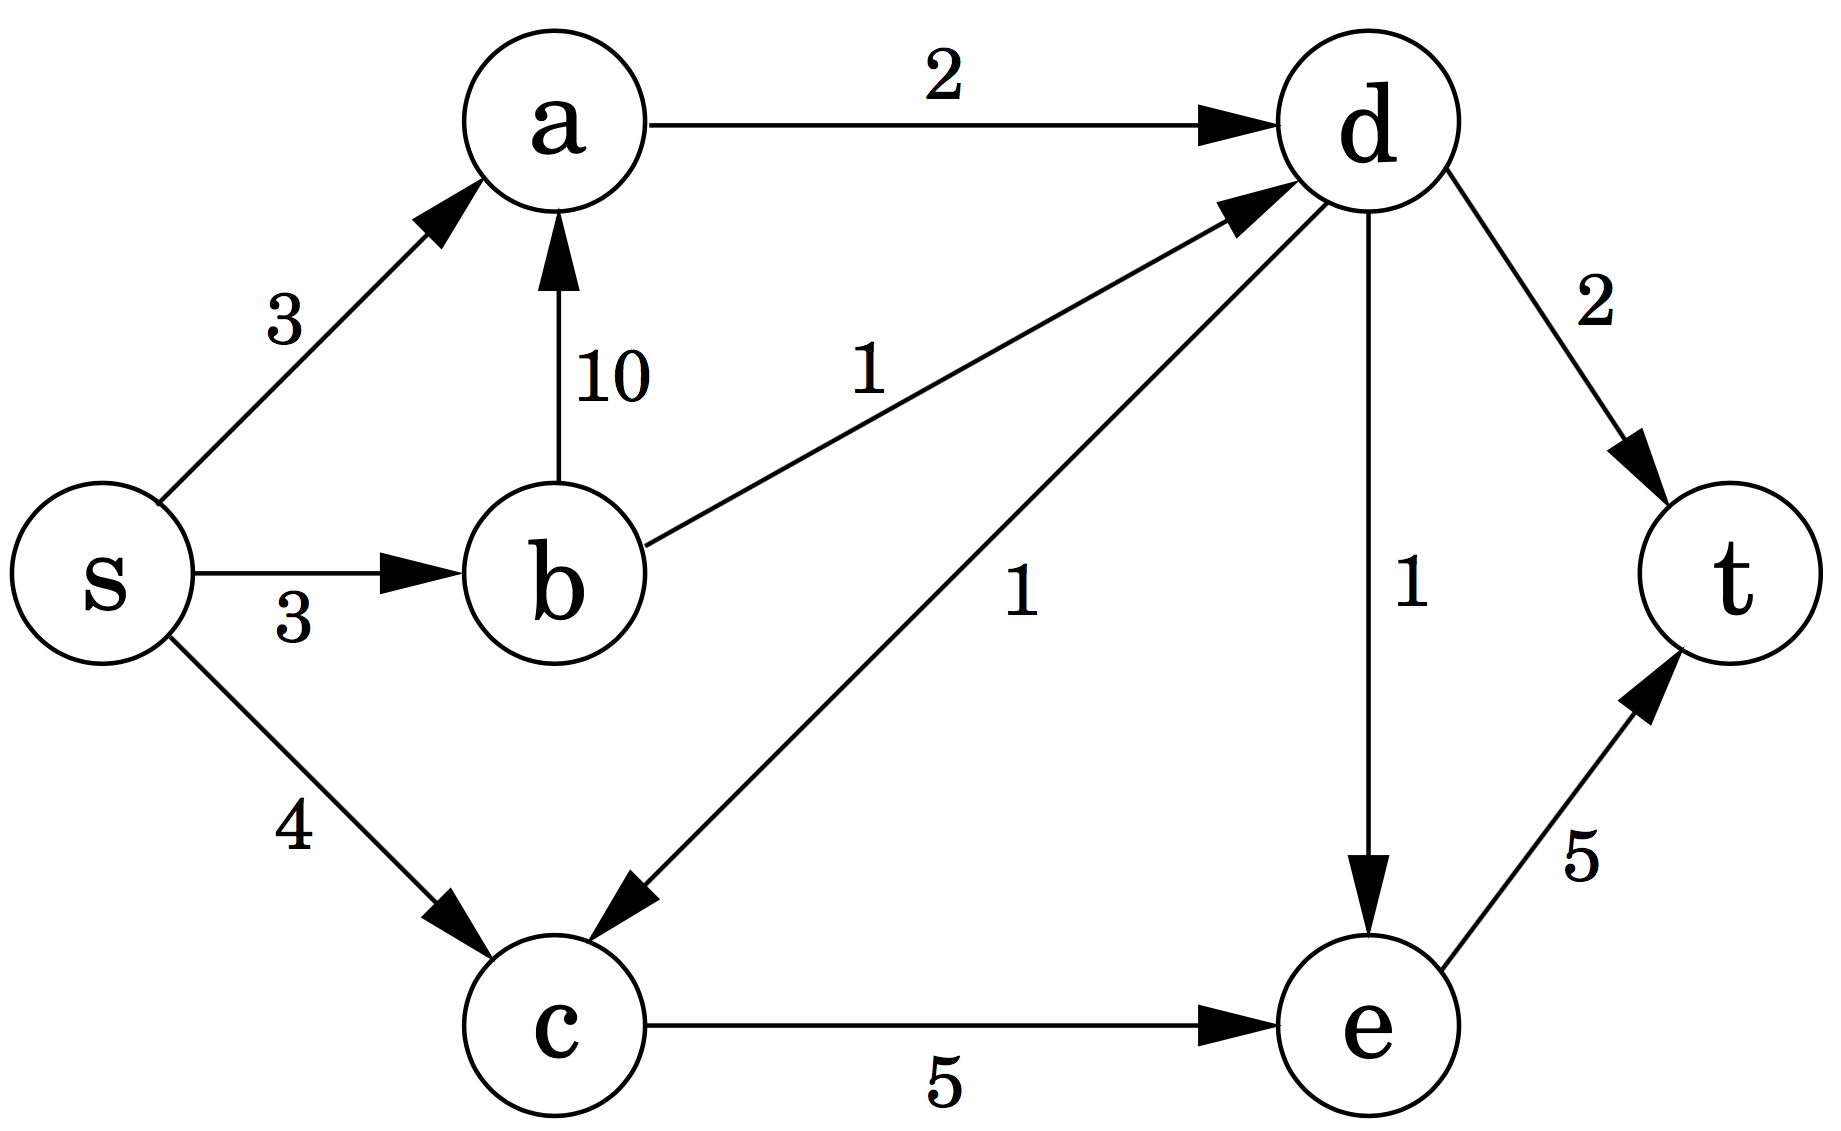
\includegraphics[width=3.7cm]{fn.png} \hspace{0.3cm}
        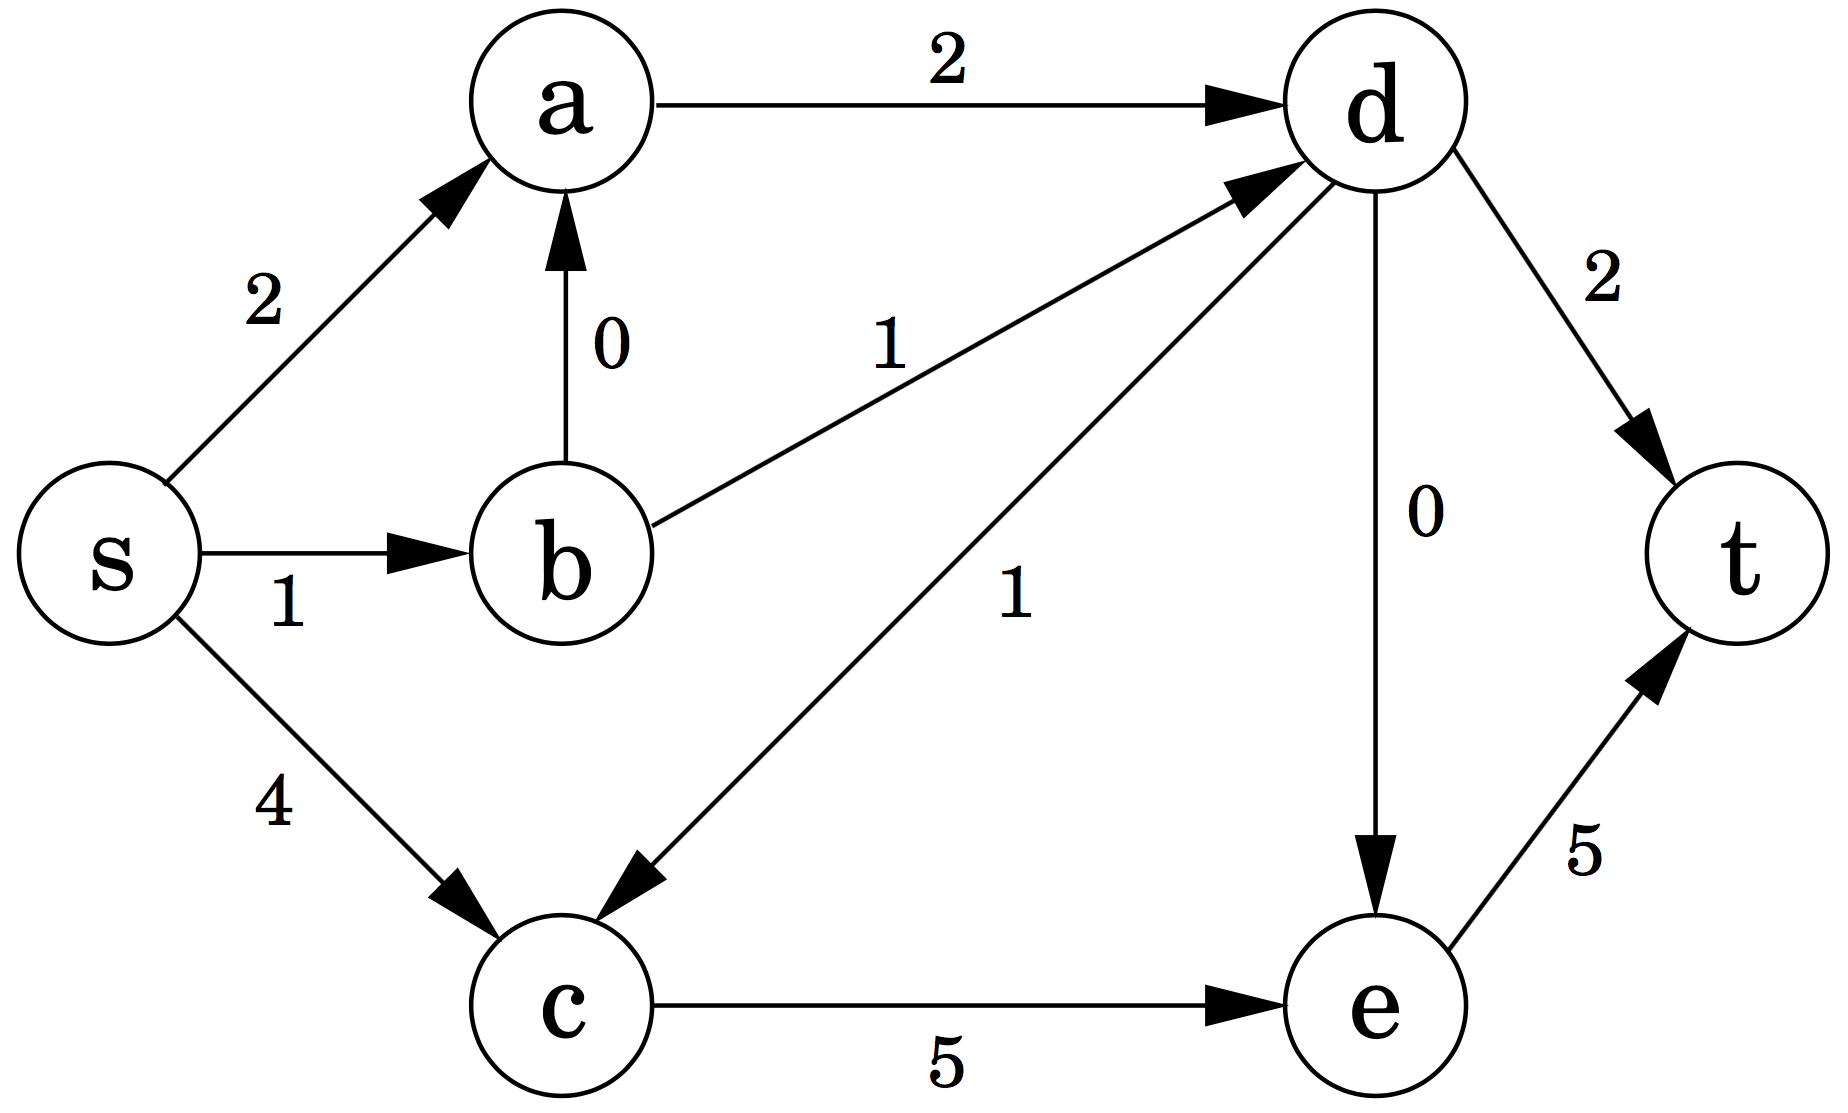
\includegraphics[width=3.7cm]{maxflow.png}
        \end{center}     
        
        \item By simulating the behavior of simplex on the linear program, we get a direct algorithm for solving max-flow. Define the \textit{residual} network $G^f=(V,E^f)$ for a flow $f$ as consisting of forward edges of capacity $c_e - f_e$ (capacity minus current flow) and back edges of capacity $f_e$ (current flow). 
        % For example, a flow network (with edges labelled $f_e / c_e$) and its residual is shown below.
        % \begin{align*}
        % 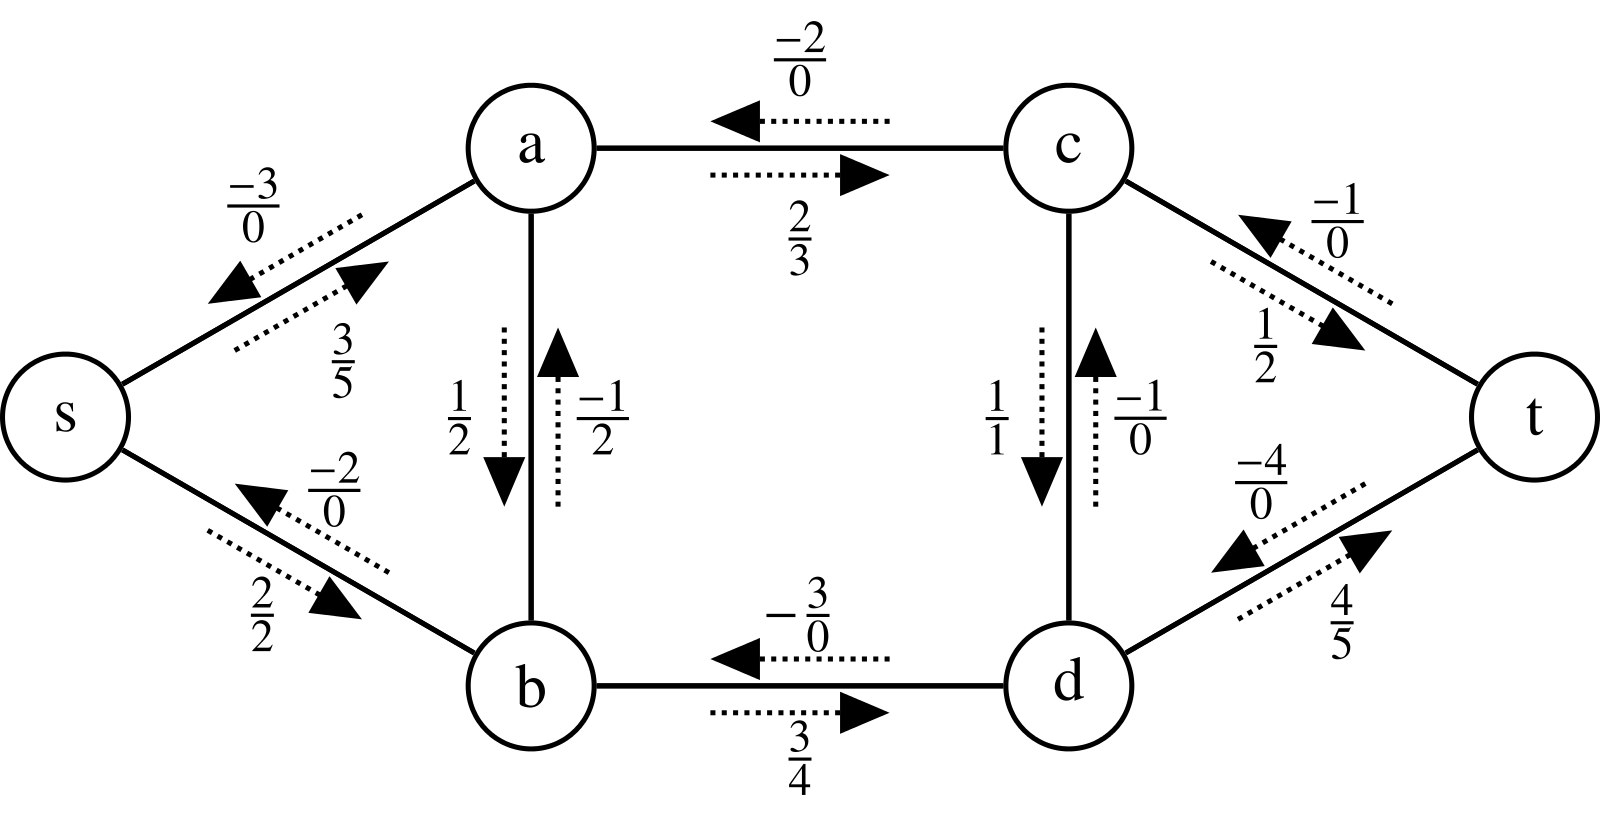
\includegraphics[width=5cm]{fn2.png} \\
        % 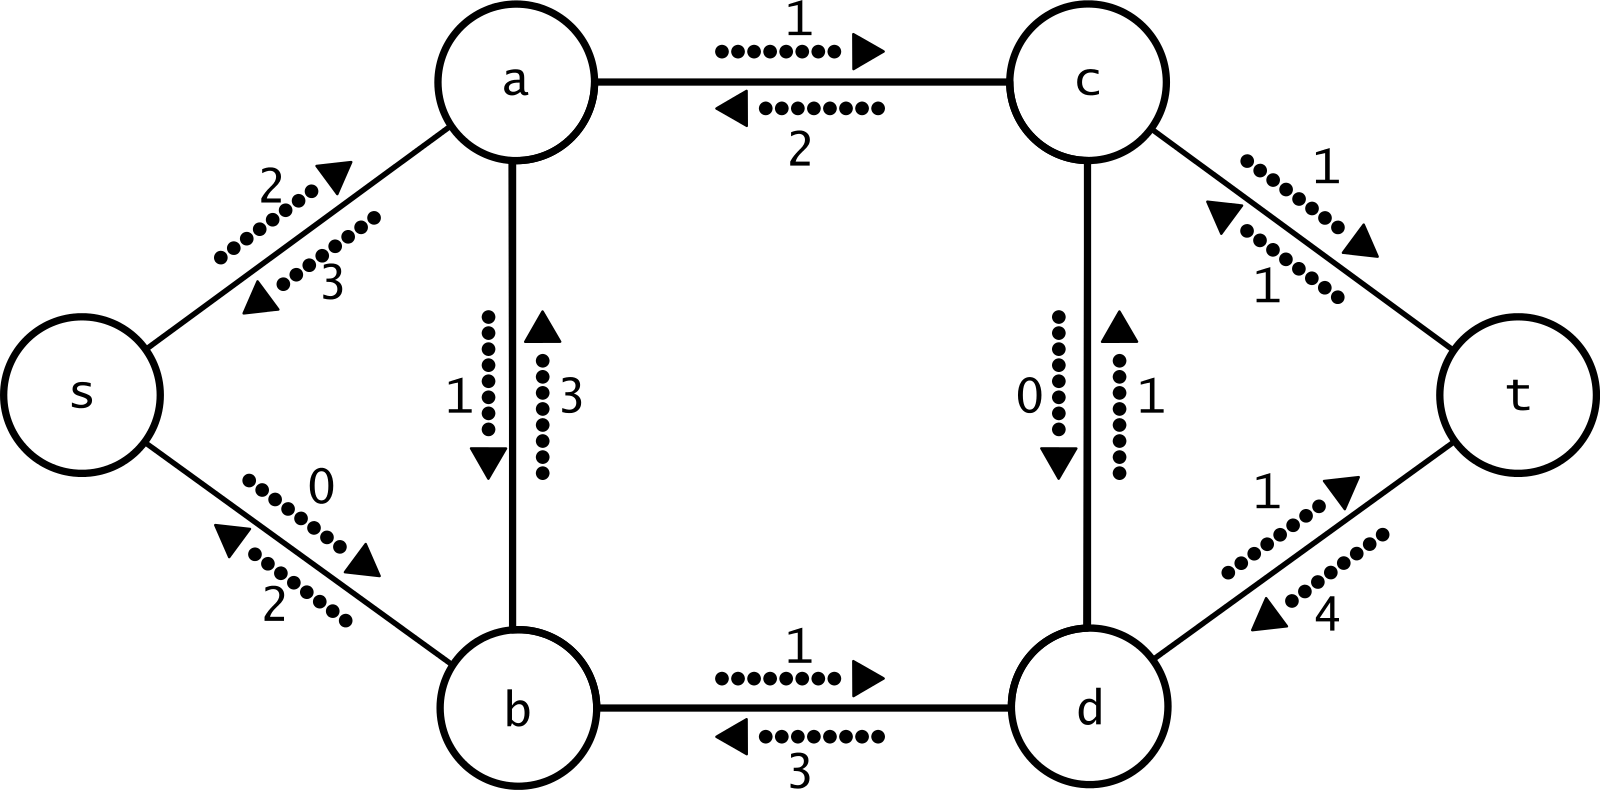
\includegraphics[width=5cm]{fn2re.png}
        % \end{align*}          
        
        \item The Ford-Fulkerson method works as follows: Start with zero flow. Find a path from $s$ to $t$ in $G^f$ such that all edge weights are greater than zero. Find the edge in the path of minimum capacity (the bottleneck), then add flow onto all edges in the path up to the capacity not being used by the bottleneck edge. Create a new residual graph and repeat until no path can be found. 
        \item An \textit{$(s,t)$-cut} partitions vertices into disjoint sets $L$ and $R$ such that $s \in L$ and $t \in R$. Its \textit{capacity} is the total capacity of the edges from $L$ to $R$, and is an upper bound on any valid flow. 
        \item \textit{Max flow min cut theorem:} The size of the maximum flow in a network equals the capacity of the smallest $(s, t)$-cut. (The two problems are dual to each other.)
        \item This min cut is found by the Ford-Fulkerson algorithm. Let $f$ be the final flow when the algorithm terminates. The min cut is given by $L$ and $R$, where $L$ is the set of nodes reachable from $s$ in $G^f$ and $R = V - L$. 
    
        \item Each iteration of the algorithm can be done in $O(|E|)$ time via DFS or BFS on $G^f$. For integer capacities, the running time is bounded by $O(C|E|)$ where $C$ is highest capacity in the network. By using BFS to find the paths, the running time is at most $O(|V| \cdot |E|^2)$ (Edmonds–Karp algorithm).
        
        \item If all edge capacities are integers, then the optimal flow found by the algorithm is integral.
        
        \item In \textit{bipartite matching}, we have a bipartite graph $G=(V=(X,Y),E)$. We wish to find a \textit{perfect matching}, that is, a matching such that every vertex in $V$ is incident to exactly one edge to a vertex in $Y$. This reduces to max flow if the graph is unweighted. 
        
        \item For example, let $X$ and $Y$ represent boys and girls, respectively. There is an edge between a boy and girl if they like each other. Create a source node $s$ with an edge to every vertex in $X$ and a sink node $t$ with with edges from every vertex in $Y$, and direct all the edges in the original graph from $X$ to $Y$. Give every edge capacity 1. There is a perfect matching if and only if the network has a flow whose size equals the number of couples. Using the algorithm above, we obtain the optimum \textit{integer}-valued flow that corresponds to the optimum matching.
    \end{enumerate}
    
    \vspace{-0.4cm}
    \subsection{Zero-Sum Games}
    \vspace{-0.2cm}
    \begin{enumerate}[label=(\alph*)]
        \item A zero-sum game is a representation of a situation in which each player's gain or loss is exactly balanced by the losses or gains of the other players.
        \item A two-player zero-sum game can be represented by a payoff matrix $G$. For example, for rock-paper-scissors with players Row and Column:
        \begin{align*}
        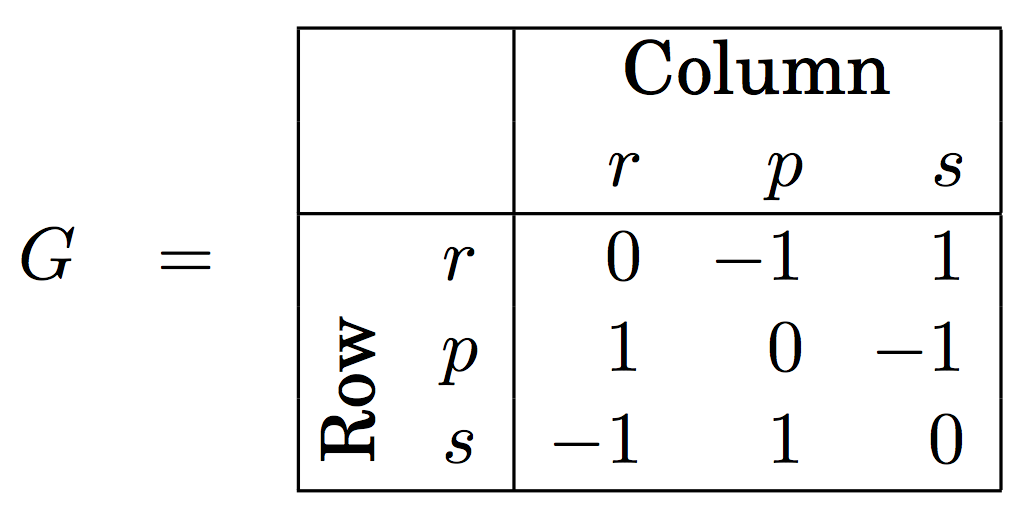
\includegraphics[width=3.5cm]{payoff_matrix.png}
        \end{align*}
        Here the entries represent Row's gain for each possible move in $\{r,p,s\}$. Row's and Column's \textit{strategy} can be denoted by the vectors $x$ and $y$, respectively, where $x_i$ is the probability that Row will play the $i$-th move (similarly for Column).
        \item The \textit{expected payoff} of the game is $\sum_{i,j} G_{ij} x_i y_j$. Row seeks to maximize this, while Column seeks to minimize this. Both cases are linear programs, and they are dual to each other.
        \item By the \textit{min-max} theorem,
        \begin{align*}
        \max_x \min_y \sum_{i,j} G_{ij} x_i y_j = \min_y \max_x \sum_{i,j} G_{ij} x_i y_j
        \end{align*}
        This shows the existence of mixed strategies that are optimal for both players and achieve the same optimal value, called the \textit{value} of the game.
    \end{enumerate}    
\end{addmargin}

\vspace{-0.2cm}
\section{NP-Complete Problems}
\vspace{-0.2cm}
\begin{addmargin}[0.8em]{0.5em}
Most of the algorithms studied thus far are efficient because their time requirement grows as a \textit{polynomial} function of the size of their input. We now explore problems for which this seems impossible.
    \subsection{Search Problems}
    \vspace{-0.2cm}
    \begin{enumerate}[label=(\alph*)]
        \item A \textit{search problem} is specified by an algorithm $\mathcal{C}$ that takes two inputs, and instance $I$ and proposed solution $S$, and runs in time polynomial in $|I|$. $S$ is a solution if $\mathcal{C}(I,S)$ is true.
        \item A \textit{Turing} reduction from $A$ to $B$ is an algorithm that solves $A$ in a polynomial number of ``steps", each of which may involve a call to a solver of $B$. 
        \item Many of the problems that follow can be formulated as a decision, search, or optimization problem. For NP-complete problems, all of these variants are \emph{equivalent} in that they reduce to each other. A common pattern is that \textsc{search} reduces to \textsc{decision} by calling the \textsc{decision} solver $O(n)$ times, and \textsc{optimization} reduces to \textsc{search} by doing binary search on the \textsc{search} solver. 
    \end{enumerate}
    
    \vspace{-0.2cm}
    \subsection{Complexity Classes}
    \vspace{-0.2cm}
    \begin{enumerate}[label=(\alph*)]
    \item \textbf{NP} is the class of all search problems, or problems for which a given solution can be verified as a solution in polynomial time.
    \item \textbf{P} is the class of all search problems that can be solved in polynomial time. These are generally problems with efficient solutions, or are ``tractable".
    \item The \textbf{P $=$ NP} question asks whether every problem whose solution can be verified in polynomial time can also be solved in polynomial time. It is widely believed \textbf{P $\neq$ NP}, but it remains one of the most important unsolved problems in mathematics.    
    \item \textbf{NP}-hard is the class of problems to which all problems in \textbf{NP} reduce. They need not be in \textbf{NP}.
    \item \textbf{NP}-complete is the class of problems that are \textbf{NP}-hard and also in \textbf{NP}. \textbf{NP}-complete problems represent the hardest problems in \textbf{NP}. 
    
    \vspace{-0.2cm}
    \begin{center}
    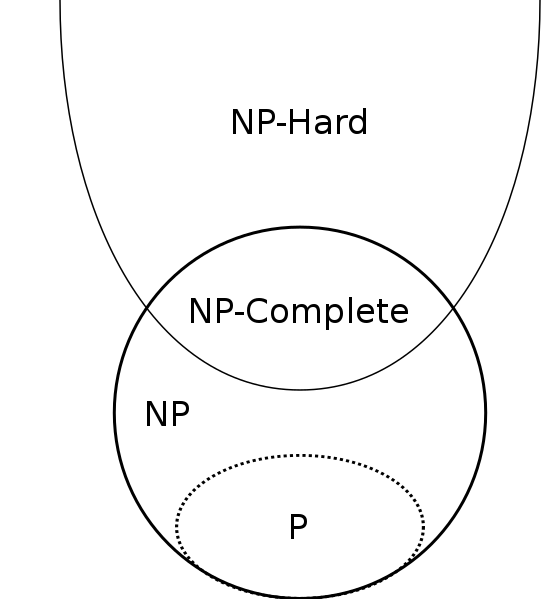
\includegraphics[width=3cm]{np_euler.png}
    \end{center}
    \vspace{-0.4cm}
    % \item Reductions are powerful tools for proving NP-completeness because they compose: if $A \rightarrow B$ and $B \rightarrow C$, then $A \rightarrow C$.
    \end{enumerate}
    
    \vspace{-0.4cm}
    \subsection{Examples of NP-Complete Problems}
    \vspace{-0.2cm}
    \begin{enumerate}[label=(\alph*)]
        \item \textsc{Satisfiability}, or \textsc{sat}, is the problem of finding a satisfying truth assignment that satisfies a given Boolean formula, or reporting that none exists. It is a canonically hard problem and was the first problem to be proven NP-complete.
        
        Certain variants of \textsc{sat} do have good algorithms (e.g. HornSat). If all clauses have only two literals (\textsc{2sat}), it can be solved in linear time. 
        
        \item A \textit{cut} is a set of edges whose removal leaves a graph disconnected. The \textsc{minimum cut} problem is as follows: given a graph with $n$ vertices and a budget $b$, find a cut with at most $b$ edges. This can be solved in polynomial time with $n - 1$ max-flow computations.
        
        \item The minimum cut often partitions a graph into a singleton vertex on one side. The \textsc{balanced cut} problem (which is NP-complete) is as follows: given a graph with $n$ vertices and a budget $b$, partition the vertices into two sets $S$ and $T$ such that $|S|,|T| \geq n / 3$ and there are at most $b$ edges between $S$ and $T$.        
        
        \item \textsc{Euler path} is the problem of finding a path in a graph that contains each \textit{edge} exactly once. Euler observed that such a path exists iff the graph is connected and every vertex (with the possible exception of the start and end vertices of the walk), has even degree. It can be solved in polynomial time.
        
        \item In contrast, \textsc{rudrata cycle} (or Hamiltonian cycle) is the problem of finding a cycle in a graph that visits each \textit{vertex} exactly once. Both the \textsc{rudrata cycle} and \textsc{rudrata path} problems are NP-complete.
        
        \item \textsc{3D matching} is a generalization of bipartite matching. Formally, let $X$, $Y$, and $Z$ be disjoint sets each of size $n$, and let $T$ consist of triples $(x, y, z)$ s.t. $x \in X, y \in Y$, and $z \in Z$  (``compatibilities" among them). $M \subseteq T$ is a 3D matching if it consists of $n$ disjoint triples. It is also NP-complete.
        
        \item \textsc{integer linear programming} is NP-complete. An important special case is \textsc{zero-one equations (zoe)}: find a vector $x$ of 0's and 1's satisfying $Ax=\vec{1}$, where $A \in \mathbb{R}^{m \times n}$ with entries in $\{0,1\}$ and $\vec{1}$ is the $m$-vector of all ones.
        
        \item Two previously seen problems, \textsc{independent set} for general graphs and \textsc{set cover} are also NP-complete. The \textsc{vertex cover} of a graph is a set of vertices such that each edge of the graph is incident to at least one vertex of the set. As special case of \textsc{set cover}, \textsc{vertex cover} is also NP-complete.
        
        \item A \textit{clique} is a subset of vertices of an undirected graph such that every two distinct vertices in the clique are adjacent (i.e. a subgraph that is \textit{complete}). The task of finding whether there is a clique of a given size in a graph, \textsc{clique}, is NP-complete.
        
        \item The \textsc{longest path} problem is to find the longest simple path (no repeated vertices) from $s$ to $t$ with weight at least $g$. It is NP-complete, which can be shown by simple reduction from \textsc{rudrata path}. 
        
        Intuitively, the longest path in $G$ corresponds to the shortest path in $-G$ (all edge weights negated), so unless $G$ is a DAG, then $-G$ contains negative cycles.
        
        \item \textsc{subset sum} is as follows: given a set of integers, find a subset whose sum is exactly $W$. As a special case of knapsack, it is also NP-complete.
        \vspace{-0.2cm}
        \begin{center}
        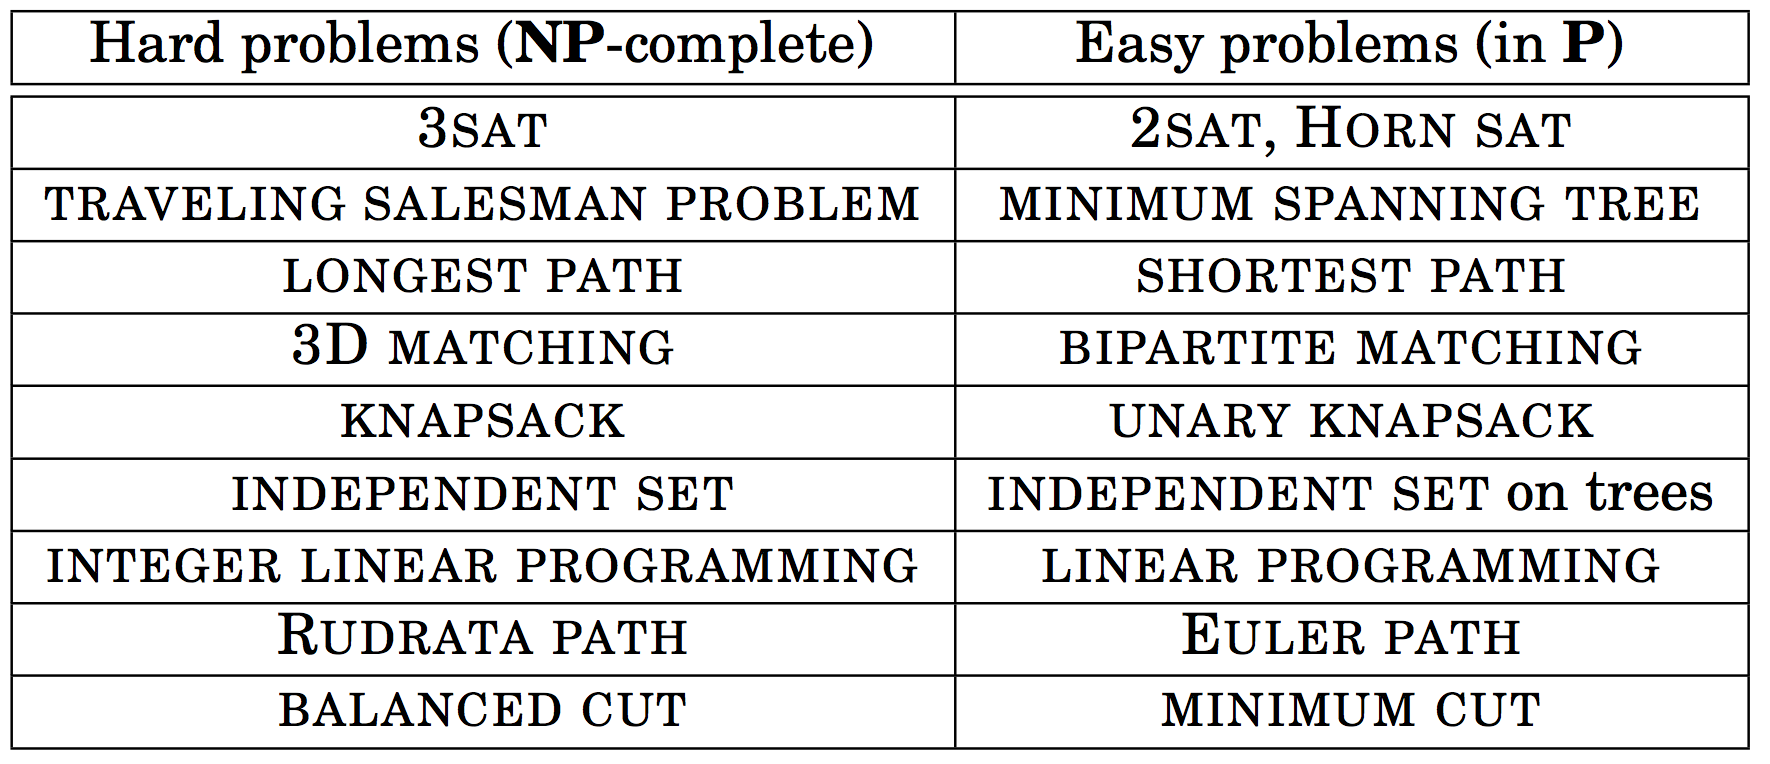
\includegraphics[width=8cm]{np_complete.png}
        \end{center}
    \end{enumerate}
    
    \vspace{-0.4cm}
    \subsection{NP-Complete Reductions}
    \vspace{-0.2cm}
    \begin{enumerate}[label=(\alph*)]
        \item A \textit{Karp} reduction from search problem $A$ to search problem $B$ is a polynomial-time algorithm $f$ that transforms any instance $I$ of $A$ into an instance $f(I)$ of $B$, together with another polynomial-time algorithm $h$ that maps any solution $S$ of $f(I)$ back into a solution $h(S)$ of $I$. They are more limited than Turing reductions (since the solver for $B$ can only be called once), but they suffice for most NP-completeness proofs.        
        \item A proof of NP-completeness for problem $B$ requires showing that (1) $B \in$ \textbf{NP}; (2) an NP-complete problem $A$ can be reduced to $B$; (3) the reduction takes polynomial time; and (4) $B$ has a solution iff $A$ has a solution.
        
        \begin{center}
        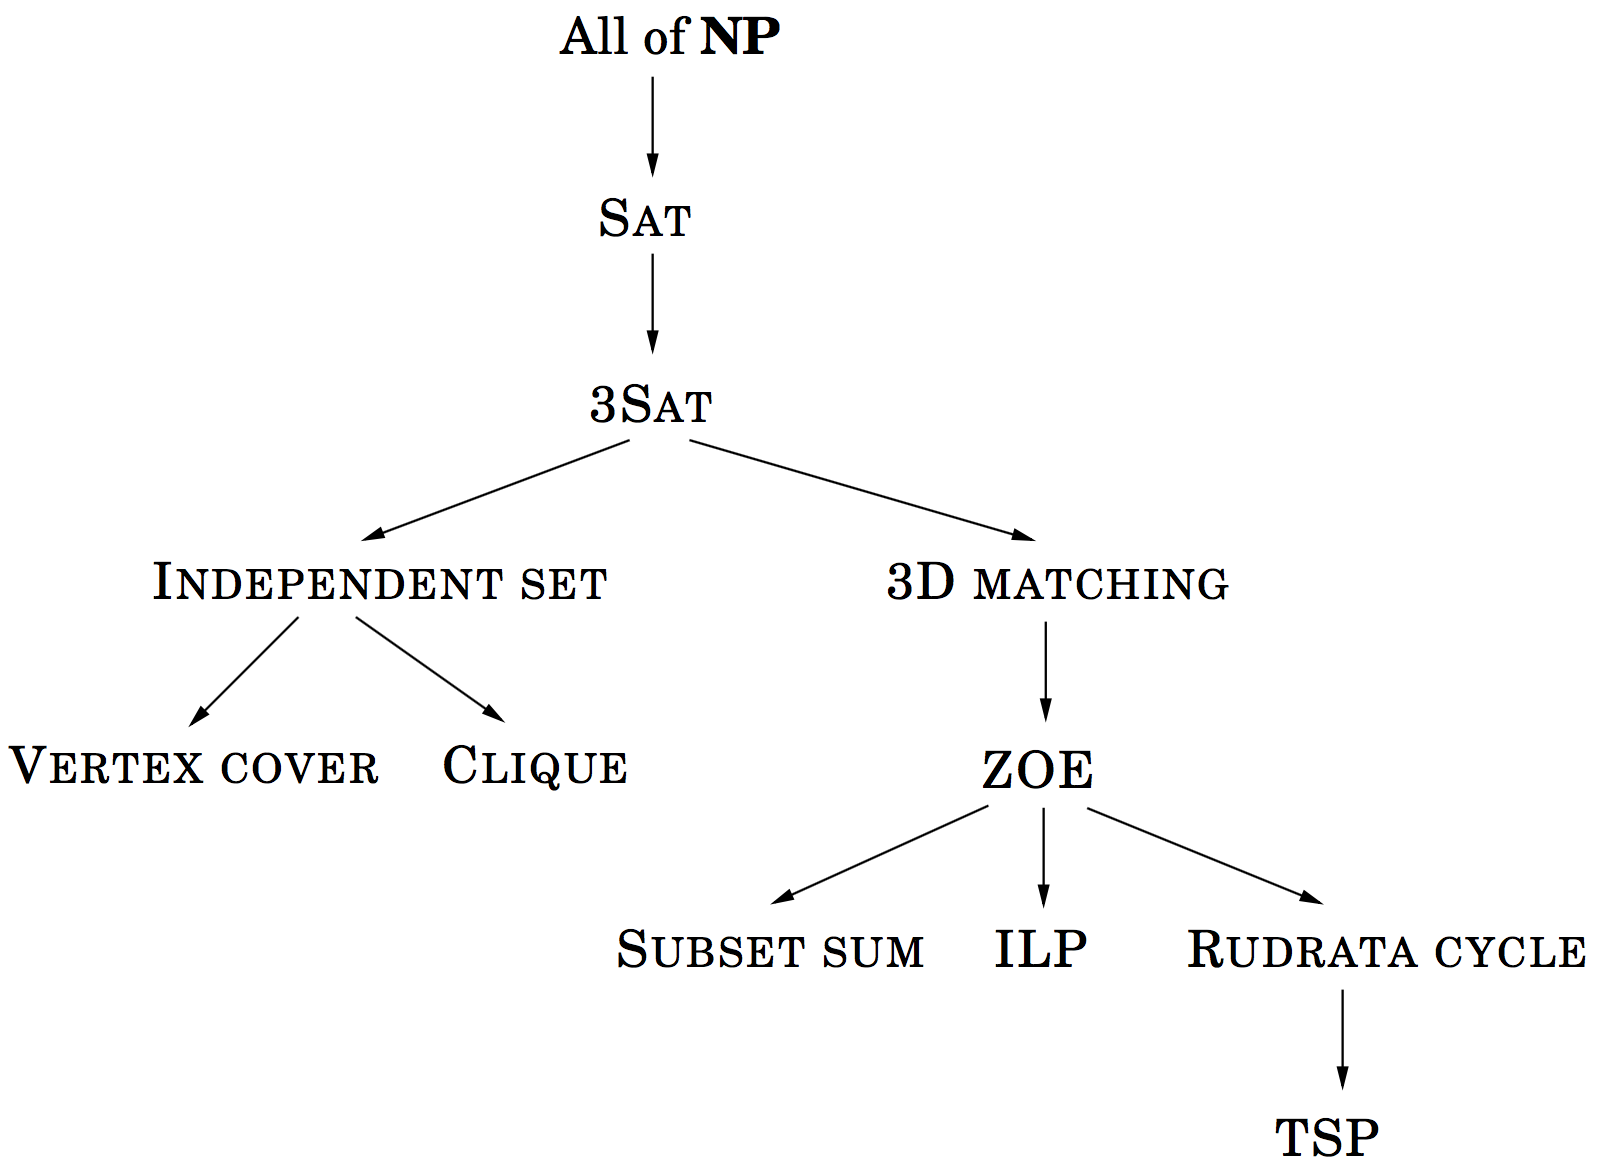
\includegraphics[width=6cm]{reductions.png}
        \end{center}         
        
        \item \textsc{3Sat} $\rightarrow$ \textsc{Independent set} \\
        In \textsc{3Sat}, we are given a conjunction (\textsc{and}) of clauses where each clause is a disjunction (\textsc{or}) of at most 3 literals. Given an instance of \textsc{3Sat}, we create an instance $(G, g)$ of \textsc{Independent set} as follows. Graph $G$ has a triangle for each clause (or just an edge if only two literals), with vertices labeled by the clause’s literals, and has additional edges between any two vertices that represent opposite literals. The goal $g$ is set to the number of clauses.
        
        \item \textsc{Sat} $\rightarrow$ \textsc{3Sat} \\
        Given an instance of \textsc{Sat}, we use the same instance for \textsc{3Sat} except that any clause $(a_1 \lor \hdots \lor a_k)$, where $k > 3$, is replaced by
        $$
        (a_1 \lor a_2 \lor y_1)(\bar{y}_1 \lor a_3 \lor y_2)(\bar{y}_2 \lor a_4 \lor y_3) \cdots (\bar{y}_{k-3} \lor a_{k-1} \lor a_k)
        $$
        The original clause is satisfied iff there is a setting of the $y_i$'s for which the new expression is satisfied. To see this, suppose the clauses in the new expression were are all satisfied. Then at least one of the literals $a_1, \hdots, a_k$ must be True, otherwise $y_1$ would have to be true, which would in turn force $y_2$ to be True, and so on, eventually falsifying the last clause. Conversely, if $(a_1 \lor \hdots \lor a_k)$ is satisfied, then some $a_i$ must be true. Setting $y_1, \hdots, y_{i-2}$ to True and the rest to False ensures all clauses are satisfied.
        
        \item \textsc{Independent set} $\rightarrow$ \textsc{Clique} \\
        Define the complement of a graph $G=(V,E)$ to be $\bar{G}=(V,\bar{E})$, where $\bar{E}$ contains precisely those pairs of vertices that are not in $E$. Then a set of vertices $S$ is an independent set of $G$ iff $S$ is a clique of $\bar{G}$. That is, vertices have no edges between them in $G$ iff they have all possible edges between them in $\bar{G}$.
        
        \item \textsc{Independent set} $\rightarrow$ \textsc{Vertex Cover} \\
        A subset $S \subseteq V$ is a vertex cover of $G=(V,E)$ iff the remaining vertices $V - S$ are an independent set.         
        
        \item \textsc{3D Matching} $\rightarrow$ \textsc{ZOE} \\
        We can think of the $0 - 1$ variables as describing a solution, and we write equations expressing the constraints of the problem. For an instance of \textsc{3D Matching} with $X,Y,Z$ each of size $n$ and $m$ triples, we have variables $x_1, \hdots, x_n$, where $x_i=1$ if the $i$th triple is chosen for the matching (and 0 otherwise). Then for each $x \in X$ (or $y \in Y$, $z \in Z$) suppose the triples containing $x$ are those numbered $j_1, \hdots, j_k$; the appropriate constraint is $x_{j_1} + \hdots x_{j_k} = 1$ which states that exactly one of these triples must be included in the matching. 
        
        \item \textsc{ZOE} $\rightarrow$ \textsc{Subset Sum} \\
        \textsc{ZOE} seeks to find a subset of columns of $A$ that sum to $\vec{1}$. Treating the columns of $A$ and the 1-vector as integers in base $n+1$ (read from top to bottom), this is an instance of \textsc{Subset Sum}. Note that we use base $n+1$ to avoid carrying in addition.
        
        \item \textsc{ZOE} $\rightarrow$ \textsc{ILP} \\
        To convert an instance $Ax = \vec{1}$ into $Ax \leq b$, simply rewrite each equation as two inequalities and add to each variable the inequalities $x_i \leq 1$ and $-x_i \leq 0$.
        
        \item \textsc{Rudrata cycle} $\rightarrow$ \textsc{TSP} \\
        For a graph $G$, construct an instance of \textsc{TSP} by letting the set of cities be $V$, the distance between cities $u$ and $v$ be $1$ if $(u,v)$ is an edge of $G$ and $2$ otherwise, and set the budget of the \textsc{TSP} instance equal to $|V|$.
        
        \item All of \textbf{NP} $\rightarrow$ \textsc{Sat}: \\
        In \textsc{Circuit Sat}, we are given a Boolean circuit: a DAG whose vertices are gates of 5 different types: \textsc{AND} and \textsc{OR} gates with indegree 2; \textsc{NOT} gates of indegree 1; \textit{known} input gates labeled True or False with no incoming edges; and \textit{unknown} input gates labeled ``?" with no incoming edges. One of the sinks of the DAG is designated as the output. As a search problem, \textsc{Circuit Sat} is: given a circuit, find an assignment to the unknown inputs such that the output gate evaluates to True, or report that no such assignment exists. \textsc{Sat} clearly reduces to \textsc{Circuit Sat}. To see the opposite direction, for each gate $g$ in the circuit, create a variable $g$ and the model the behavior of the gate as follows:
        \begin{center}
        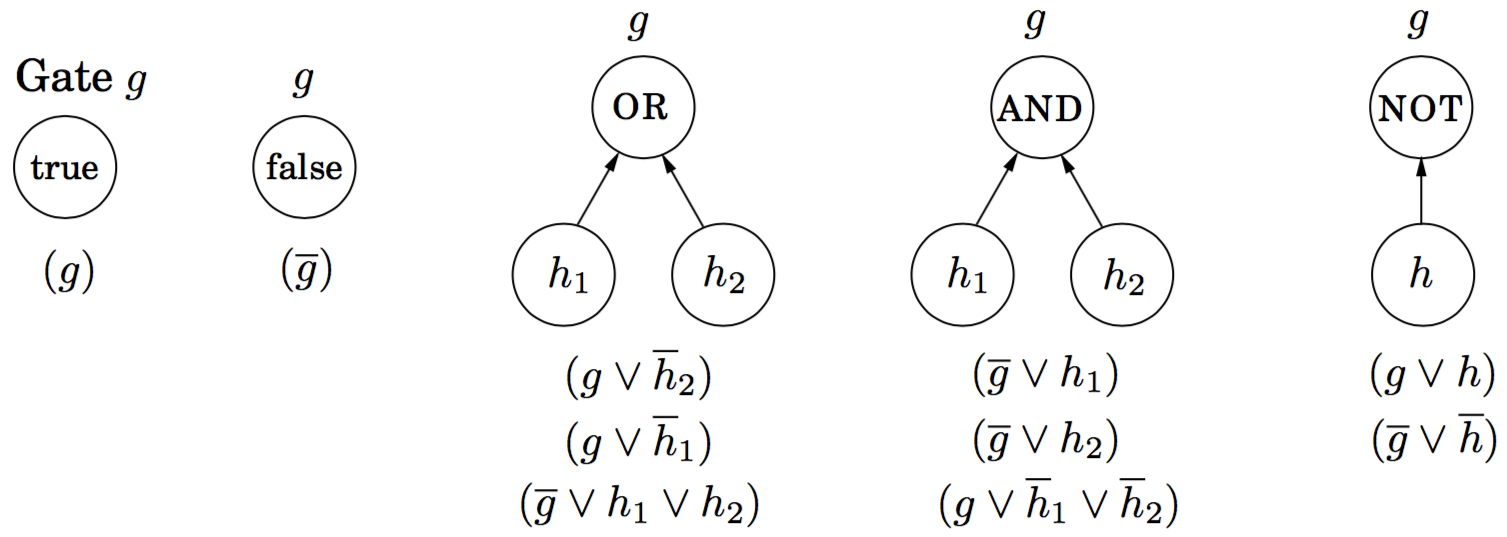
\includegraphics[width=6.5cm]{circuit_sat.png}
        \end{center}
        Given any instance $I$ of problem $A$, we can construct in polynomial time a circuit whose known inputs are the bits of $I$, and whose unknown inputs are the bits of $S$, such that the output is True iff the unknown inputs spell a solution of $I$.
        
    \end{enumerate}    
\end{addmargin}

\section{Coping with NP-Completeness}
\begin{addmargin}[0.8em]{0.5em}
The vast expanse of search problems is NP-complete. Most modern research on algorithms and complexity focuses on dealing with the difficulty of these problems.
    \subsection{Intelligent Exhaustive Search}
    \begin{enumerate}[label=(\alph*)]
        \item \textbf{Backtracking} is a general algorithm that incrementally builds candidate solutions where partial assignments can be quickly discarded if they cannot possibly yield a valid solution. A backtracking algorithm requires a test that quickly declares a partial assignment to be one of three outcomes: failure, success, or uncertainty. With the right test, expand, and choose routines, backtracking can be very effective in practice, especially in satisfiability programs.
        
        \item \textbf{Branch-and-bound} generalizes backtracking to optimization problems. A partial solution is rejected if its cost exceeds that of some other solution already encountered. Since the cost is generally not efficiently computable, a lower bound is used. For example, in \textsc{TSP}, a partial solution is a simple path $a \to b$ passing through some vertices $S \subseteq V$, where $a,b \in S$. At each step of the branch-and-bound algorithm, we extend a particular partial solution by a single edge $(b,x)$, where $x \in V-S$. A lower bound is the sum of the following: the lightest edge from $a$ to $V - S$; the lightest edge from $b$ to $V - S$; and the MST of $V - S$.
    \end{enumerate}
    \vspace{-0.6cm}
    \subsection{Approximation Algorithms}
    \vspace{-0.2cm}
    \begin{enumerate}[label=(\alph*)]
        \item Let $\mathcal{A}$ be an algorithm for a general minimization problem which, given an instance $I$, returns a solution with value $\mathcal{A}(I)$. Let $\textsc{opt}(I)$ denote the value of the optimum solution to $I$. The approximation ratio of algorithm $\mathcal{A}$ is 
        $$
        \alpha_\mathcal{A} = \max_I \frac{\mathcal{A}(I)}{\textsc{opt}(I)}
        $$
        i.e., the factor by which the output of $\mathcal{A}$ exceeds the optimal solution, on the worst-case input. For example, we have already seen a greedy algorithm for \textsc{Set cover} with approximation ratio $\log{n}$. Note that $\alpha_\mathcal{A}$ is defined as the reciprocal for maximization problems.
        
        \item A 2-approximation to \textsc{Vertex cover} is based on the notion of a \textit{matching}, or a subset of edges that have no vertices in common. A matching is maximal if no more edges can be added to it. They are simple to compute: repeatedly pick edges that are disjoint from the ones chosen already. Any vertex cover of a graph $G$ must be at least as large as the number of edges in any matching in $G$. The algorithm is to find a maximal matching $M \subseteq E$ and return all vertices that are endpoints in $M$ (at most $2|M|$ vertices).
        
        \item In a \textit{clustering} problem, we have high-dimensional data we wish to divide into groups. Assume we have a distance metric $d$ satisfying
        \begin{itemize}
        \item $d(x,y) \geq 0$ for all $x,y$
        \item $d(x,y) = 0$ iff $x=y$
        \item $d(x,y) = d(y,x)$
        \item $d(x,y) \leq d(x,z) + d(z,y)$ (Triangle inequality)
        \end{itemize}
        
        \item $k$-\textsc{cluster} \\
        \textit{Input:} Data points $X = \{ x_1, \hdots, x_n \}$ with distance metric $d(\cdot, \cdot)$; integer $k$.
        
        \textit{Output:} Partition of $X$ into $k$ clusters $C_1, \hdots, C_k$. 
        
        \textit{Goal:} Minimize diameter of clusters,
        $$
        \max_{j} \max_{x_a, x_b \in C_j} d(x_a, x_b).
        $$
        
        $k$-\textsc{cluster} (also called $k$-means clustering) is NP-hard, but there are efficient heuristic algorithms. A simple 2-approximation is as follows:
        \begin{minted}[linenos=false, escapeinside=||, mathescape=true]{octave}
function kClusterApprox(|$X$|)
|$\mu_1$| = random(|$X$|)
for |$i=2$| to |$k$|:
    # point farthest from $\mu_1, \hdots, \mu_{i-1}$
    |$\mu_i$| = argmax(|$\min_{j < i} d(\cdot, \mu_j)$|)
for |$i=1$| to |$k$|:
    |$C_i$| = |$ \{ x \in X \text{ whose closest center is } \mu_i \}$|
return |$C_1, \hdots, C_k$|
        \end{minted}        
        Let $x \in X$ be the point farthest from $\mu_1, \hdots, \mu_k$, and let $r$ be its distance from the closest center. Every point in $X$ must be within distance $r$ of its cluster center, so every cluster has diameter at most $2r$. Furthermore, we have identified $k+1$ points $\{ \mu_1, \hdots, \mu_k, x\}$ that are at distance at least $r$ away from each other. Any partition into $k$ clusters must put two of these points in the same cluster and must therefore have diameter at least $r$.
        
        \item A simple 2-approximation to \textsc{TSP} is based on MSTs. Removing any edge from a TSP tour leaves a path through all the vertices, which is a spanning tree. The TSP tour cost is thus \textit{at least} the MST cost. We construct a TSP tour from a MST by traversing each edge twice (which is at most twice the optimal cost). The tour must ``shortcut" any city it is about to revisit for the next new city. By the triangle inequality, these bypasses can only make the overall tour shorter.
        
        There is no polynomial-time finite approximation for general TSP, in which there is no metric. 
        The idea is to alter the reduction given in \textsc{Rudrata Cycle} $\rightarrow$ \textsc{TSP} by replacing the edge weight 2 with a specific (large) value so that any approximate solution solves the decision problem of Rudrata path.
        
        \item We now consider an approximation to \textsc{knapsack}. Using similar techniques to the $O(nW)$ DP algorithm, there is a $O(nV)$ DP algorithm where $V$ is the sum of values of the items. The idea is to scale the values down by some $\epsilon > 0$:
        \begin{minted}[linenos=false, escapeinside=??, mathescape=true]{octave}
function knapsackApprox(?$w[1 \cdots n], v[1 \cdots n], W$?)
discard any item with weight ?$> W$?
?$v_{\text{max}}$? = max?$_i$? ?$v_i$?
for ?$i=1$? to ?$n$?:
    ?$\widehat{v}_i$? = ?$\lfloor v_i \cdot \frac{n}{\epsilon \cdot v_{\text{max}}} \rfloor$? # rescale values
return knapsackDP(?$w[1 \cdots n], \widehat{v}[1 \cdots n], W$?)
        \end{minted}   
        The rescaled values $\widehat{v}_i$ are all at most $n/\epsilon$, so the DP algorithm is $O(n^3 / \epsilon)$. It can be shown that it will return a solution at least $(1 - \epsilon)$ times the optimal value.
        
        \item NP-complete optimization problems are classified as follows: 
        \begin{itemize}
        \item those for which no finite approximation ratio is possible, e.g. general \textsc{TSP}
        \item those for which an approximation ratio is possible, but there are limits to how small it can be, e.g. \textsc{Vertex cover}, $k$-\textsc{cluster}, \textsc{TSP}
        \item those for which the approximation ratio is about $\log{n}$, e.g. \textsc{set cover}
        \item those for which approximation algorithms with arbitrarily small error exist, e.g. \textsc{knapsack}
        \end{itemize}

    \end{enumerate}    
    \vspace{-0.2cm}
    \subsection{Local search heuristics}
    \vspace{-0.2cm}
    \begin{enumerate}[label=(\alph*)]
        \item Local search is a paradigm for solving hard optimization problems. It starts with an initial solution, introduces local changes, and keeps them if they are an improvement. The current solution is iteratively replaced by a better one in its \textit{neighborhood}.
        \item For example, a local search procedure to solve \textsc{TSP} might use the 2-change neighborhood: for a tour $s$, define the neighborhood as the set of tours that can be obtained by removing two edges of $s$ and then putting in two other edges. The only guarantee is that the final tour is \textit{locally} optimal. A larger neighborhood (e.g. $k$-change) may decrease low-quality local optima, but each iteration becomes more expensive; there is a trade-off in efficiency and quality.
        \item Local optima can be dealt with by randomization and restarts. Randomization is typically used to pick a random initial solution and to choose a local move when several are available. Repeating a local search with different random seeds increases the probability of reaching a global optima. 
        \item As problem size grows, simply repeating local search is ineffective as the ratio of bad to good local optima often becomes exponentially large. \textit{Simulated annealing} is a method that occasionally allows ``downhill" moves in the hope that they will pull the search out of dead ends. It works by introducing a temperature $T$ that gradually reduces to zero. For current solution $s$ and neighbor $s'$, let $\Delta = \texttt{cost}(s') - \texttt{cost}(s)$. Simulated annealing replaces $s$ with $s'$ with probability 1 if $\Delta < 0$, else with probability $e^{-\Delta / T}$. Choosing an appropriate cooling schedule takes care, but simulated annealing in practice works remarkably well.
    \end{enumerate}     
\end{addmargin}
\vspace{-0.4cm}
\section{Special Topics - Cryptography}
\begin{addmargin}[0.8em]{0.5em}
    \subsection{Primality Testing}
    \vspace{-0.2cm}
    \begin{enumerate}[label=(\alph*)]
        \item Modern cryptography is based on the idea that factoring is hard and primality is easy. 
        \item Recall Fermat's little theorem: If $p$ is prime, then for every integer $a$, $1 \leq a < p$, 
        $$
        a^{p-1} \equiv 1\ (\text{mod}\ p)
        $$
        
        \item This suggests a primality test: for the number $N$, pick a random integer $1 \leq a < N$ and return whether or not $a^{N-1} \equiv 1\ (\text{mod}\ N)$. Although the theorem is \textit{not} an if and only if condition, \textit{most} values of $a$ will fail the test if $N$ is composite.
        
        More precisely, if $a^{N-1} \not\equiv 1\ (\text{mod}\ N)$ for some $a$ relatively prime to $N$ (i.e. the only positive integer that divides both of them is 1), then it must hold for at least half the choices of $a < N$. The probability of a false positive from Fermat's test is thus $\leq \frac{1}{2}$.
        
        The probability of error is reduced by repeating the procedure many times:
        \begin{minted}[linenos=false, escapeinside=??, mathescape=true]{octave}
function primality(?$N$?)
pick ?$a_1, \hdots, a_k \in \{ 1, 2, \hdots, N-1 \}$? at random
for ?$i=1$? to ?$k$?:
    if ?$a_i^{N-1} \equiv 1\ (\text{mod}\ N)$?:
        return True
return False
        \end{minted}     
        The probability of a false positive is at most $\frac{1}{2^k}$, which is negligible for large enough $k$.
        \item Note that there are certain extremely rare composite numbers called \textit{Carmichael numbers} that pass Fermat’s test for all $a$ relatively prime to $N$. There are ways of dealing with them.
    \end{enumerate} 
    \vspace{-0.2cm}
    \subsection{One-way functions}
    \begin{enumerate}[label=(\alph*)]
        \item A function $f : \{0, 1 \}^n \mapsto \{0, 1\}^m$ is said to be a one-way function if 
        \begin{itemize}
            \item $f$ is computable in polynomial time.
            \item Any polynomial time algorithm that attempts to invert $f$ given the image of a random input $f(x)$ succeeds with negligible probability. That is, $\forall$ PPT (probabalistic polynomial time) adversary algorithms $\mathcal{A}$ and $\forall$ $c>0$, we have $\exists$ $n_0$ s.t. $\forall n \geq n_0$
            $$
            P(\mathcal{A}(f(x)) = x) \leq \frac{1}{n^c}
            $$
        \end{itemize}
        If $f$ is addionally bijective, it is called a \textit{one-way permutation}.
        \item It is not known whether one-way functions exist. The existence of one-way functions would imply that \textbf{P} $\neq$ \textbf{NP}.
        \item Let $f : \{0, 1 \}^n \mapsto \{0, 1\}^n$ be a one-way permutation. $B : \{0, 1 \}^n \mapsto \{0, 1\}$ is a \textit{hard core bit} of $f$ if $B$ is computable in polynomial time and there is no PPT algorithm that computes $B(x)$ from $f(x)$ with a non-negligible advantage over random guess.
        \item Assuming one-way permutations exist, one application is pseudorandom generators. A \textit{pseudorandom generator} (PRG) is a deterministic procedure that maps a random seed to a longer pseudorandom string such that the output is indistinguishable from being uniformly random. 
        \item Let $f : \{0, 1 \}^n \mapsto \{0, 1\}^n$ be a one-way permutation. Construct $G: \{0, 1 \}^{2n} \mapsto \{0, 1\}^{2n+1}$ as
        $$
        G(x,r) = f(x) \| r \| B(x,r)
        $$
        where $\|$ denotes concatenation, $x,r \in \{ 0, 1 \}^n$, and $B(x,r)$ is a hard core bit for the function $f(x) \| r$ defined as
        $$
        B(x,r) = \left( \sum_{i=1}^{n} x_i r_i  \right) \, (\text{mod}\ 2)
        $$
        It can be shown that $G$ is a PRG.
    \end{enumerate}
\end{addmargin}    

% \pagebreak

% \section{Appendix: Algorithm Cheat Sheet}
% \begin{addmargin}[0.8em]{0.5em}
%     \subsection{Data Structures}
%     \begin{enumerate}[label=(\alph*)]
%         \item Coming soon: comprehensive collection of hundreds of CS170 and/or interview-style technical questions. All examples will include the main idea solution and running time (if applicable).
%         \item Implementations (in Java) of the most fundamental data structures will also be included.
%         \item The goal of this is to get in the mindset of an efficient programmer. Most problems are variants of a few clever ideas; with enough exposure, they become intuitive and one can then approach new problems with a rich toolkit of problem-solving skills they can apply.
%         \item Sources: 
%         \begin{enumerate}
%             \item Cracking the coding interview. 
%             \item CS170 discussions, homeworks, and exams. \item GeeksforGeeks.
%             \item StackOverflow
%         \end{enumerate}
%     \end{enumerate}
    
%     \subsection{Sorting Algorithms}
%     \begin{enumerate}[label=(\alph*)]
%         \item 
%     \end{enumerate}
    
%     \subsection{Search Problems}
%     \begin{enumerate}[label=(\alph*)]
%         \item 
%     \end{enumerate}
    
%     \subsection{Array Algorithms}
%     \begin{enumerate}[label=(\alph*)]
%         \item 
%     \end{enumerate}   
    
%     \subsection{String Algorithms}
%     \begin{enumerate}[label=(\alph*)]
%         \item 
%     \end{enumerate}      
    
%     \subsection{Graph Algorithms}
%     \begin{enumerate}[label=(\alph*)]
%         \item 
%     \end{enumerate}         
    
%     \subsection{Parallelism}
%     \begin{enumerate}[label=(\alph*)]
%         \item 
%     \end{enumerate}
    
%     \subsection{Basic SQL}
%     \begin{enumerate}[label=(\alph*)]
%         \item 
%     \end{enumerate}     
    

\end{multicols}
\end{document}